%%% Hlavní soubor. Zde se definují základní parametry a odkazuje se na ostatní části. %%%

%% Verze pro jednostranný tisk:
% Okraje: levý 40mm, pravý 25mm, horní a dolní 25mm
% (ale pozor, LaTeX si sám přidává 1in)
\documentclass[12pt,a4paper]{report}
\setlength\textwidth{145mm}
\setlength\textheight{247mm}
\setlength\oddsidemargin{15mm}
\setlength\evensidemargin{15mm}
\setlength\topmargin{0mm}
\setlength\headsep{0mm}
\setlength\headheight{0mm}
% \openright zařídí, aby následující text začínal na pravé straně knihy
\let\openright=\clearpage

%% Pokud tiskneme oboustranně:
% \documentclass[12pt,a4paper,twoside,openright]{report}
% \setlength\textwidth{145mm}
% \setlength\textheight{247mm}
% \setlength\oddsidemargin{14.2mm}
% \setlength\evensidemargin{0mm}
% \setlength\topmargin{0mm}
% \setlength\headsep{0mm}
% \setlength\headheight{0mm}
% \let\openright=\cleardoublepage

%% Vytváříme PDF/A-2u
\usepackage[a-2u]{pdfx}

%% Přepneme na českou sazbu a fonty Latin Modern
\usepackage[czech]{babel}
\usepackage{lmodern}
\usepackage[T1]{fontenc}
\usepackage{textcomp}

%% Použité kódování znaků: obvykle latin2, cp1250 nebo utf8:
\usepackage[utf8]{inputenc}

%%% Další užitečné balíčky (jsou součástí běžných distribucí LaTeXu)
\usepackage{amsmath}        % rozšíření pro sazbu matematiky
\usepackage{amsfonts}       % matematické fonty
\usepackage{amsthm}         % sazba vět, definic apod.
\usepackage{bbding}         % balíček s nejrůznějšími symboly
			    % (čtverečky, hvězdičky, tužtičky, nůžtičky, ...)
\usepackage{bm}             % tučné symboly (příkaz \bm)
\usepackage{graphicx}       % vkládání obrázků
\usepackage{fancyvrb}       % vylepšené prostředí pro strojové písmo
\usepackage{indentfirst}    % zavede odsazení 1. odstavce kapitoly
\usepackage{natbib}         % zajištuje možnost odkazovat na literaturu
			    % stylem AUTOR (ROK), resp. AUTOR [ČÍSLO]
\usepackage[nottoc]{tocbibind} % zajistí přidání seznamu literatury,
                            % obrázků a tabulek do obsahu
\usepackage{icomma}         % inteligetní čárka v matematickém módu
\usepackage{dcolumn}        % lepší zarovnání sloupců v tabulkách
\usepackage{booktabs}       % lepší vodorovné linky v tabulkách
\usepackage{paralist}       % lepší enumerate a itemize
\usepackage{xcolor}         % barevná sazba

%%% Údaje o práci

\def\opt{\operatorname{OPT}}

% Název práce v jazyce práce (přesně podle zadání)
\def\NazevPrace{Název práce}

% Název práce v angličtině
\def\NazevPraceEN{Name of thesis}

% Jméno autora
\def\AutorPrace{Jméno Příjmení}

% Rok odevzdání
\def\RokOdevzdani{ROK}

% Název katedry nebo ústavu, kde byla práce oficiálně zadána
% (dle Organizační struktury MFF UK, případně plný název pracoviště mimo MFF)
\def\Katedra{Název katedry nebo ústavu}
\def\KatedraEN{Name of the department}

% Jedná se o katedru (department) nebo o ústav (institute)?
\def\TypPracoviste{Katedra}
\def\TypPracovisteEN{Department}

% Vedoucí práce: Jméno a příjmení s~tituly
\def\Vedouci{Vedoucí práce}

% Pracoviště vedoucího (opět dle Organizační struktury MFF)
\def\KatedraVedouciho{katedra}
\def\KatedraVedoucihoEN{department}

% Studijní program a obor
\def\StudijniProgram{studijní program}
\def\StudijniObor{studijní obor}

% Nepovinné poděkování (vedoucímu práce, konzultantovi, tomu, kdo
% zapůjčil software, literaturu apod.)
\def\Podekovani{%
Poděkování.
}

% Abstrakt (doporučený rozsah cca 80-200 slov; nejedná se o zadání práce)
\def\Abstrakt{%
Abstrakt.
}
\def\AbstraktEN{%
Abstract.
}

% 3 až 5 klíčových slov (doporučeno), každé uzavřeno ve složených závorkách
\def\KlicovaSlova{%
{klíčová} {slova}
}
\def\KlicovaSlovaEN{%
{key} {words}
}

%% Balíček hyperref, kterým jdou vyrábět klikací odkazy v PDF,
%% ale hlavně ho používáme k uložení metadat do PDF (včetně obsahu).
%% Většinu nastavítek přednastaví balíček pdfx.
\hypersetup{unicode}
\hypersetup{breaklinks=true}

%% Definice různých užitečných maker (viz popis uvnitř souboru)
%%% Tento soubor obsahuje definice různých užitečných maker a prostředí %%%
%%% Další makra připisujte sem, ať nepřekáží v ostatních souborech.     %%%

%%% Drobné úpravy stylu

% Tato makra přesvědčují mírně ošklivým trikem LaTeX, aby hlavičky kapitol
% sázel příčetněji a nevynechával nad nimi spoustu místa. Směle ignorujte.
\makeatletter
\def\@makechapterhead#1{
  {\parindent \z@ \raggedright \normalfont
   \Huge\bfseries \thechapter. #1
   \par\nobreak
   \vskip 20\p@
}}
\def\@makeschapterhead#1{
  {\parindent \z@ \raggedright \normalfont
   \Huge\bfseries #1
   \par\nobreak
   \vskip 20\p@
}}
\makeatother

% Toto makro definuje kapitolu, která není očíslovaná, ale je uvedena v obsahu.
\def\chapwithtoc#1{
\chapter*{#1}
\addcontentsline{toc}{chapter}{#1}
}

% Trochu volnější nastavení dělení slov, než je default.
\lefthyphenmin=2
\righthyphenmin=2

% Zapne černé "slimáky" na koncích řádků, které přetekly, abychom si
% jich lépe všimli.
\overfullrule=1mm

%%% Makra pro definice, věty, tvrzení, příklady, ... (vyžaduje baliček amsthm)

\theoremstyle{plain}
\newtheorem{veta}{Věta}
\newtheorem{lemma}[veta]{Lemma}
\newtheorem{tvrz}[veta]{Tvrzení}
\newtheorem{pozorovani}[veta]{Pozorování}

\theoremstyle{plain}
\newtheorem{definice}{Definice}

\theoremstyle{remark}
\newtheorem*{dusl}{Důsledek}
\newtheorem*{pozn}{Poznámka}
\newtheorem*{prikl}{Příklad}

%%% Prostředí pro důkazy

\newenvironment{dukaz}{
  \par\medskip\noindent
  \textit{Důkaz}.
}{
\newline
\rightline{$\qedsymbol$}
}

%%% Prostředí pro sazbu kódu, případně vstupu/výstupu počítačových
%%% programů. (Vyžaduje balíček fancyvrb -- fancy verbatim.)

\DefineVerbatimEnvironment{code}{Verbatim}{fontsize=\small, frame=single}

%%% Prostor reálných, resp. přirozených čísel
\newcommand{\R}{\mathbb{R}}
\newcommand{\N}{\mathbb{N}}

%%% Užitečné operátory pro statistiku a pravděpodobnost
\DeclareMathOperator{\pr}{\textsf{P}}
\DeclareMathOperator{\E}{\textsf{E}\,}
\DeclareMathOperator{\var}{\textrm{var}}
\DeclareMathOperator{\sd}{\textrm{sd}}

%%% Příkaz pro transpozici vektoru/matice
\newcommand{\T}[1]{#1^\top}

%%% Vychytávky pro matematiku
\newcommand{\goto}{\rightarrow}
\newcommand{\gotop}{\stackrel{P}{\longrightarrow}}
\newcommand{\maon}[1]{o(n^{#1})}
\newcommand{\abs}[1]{\left|{#1}\right|}
\newcommand{\dint}{\int_0^\tau\!\!\int_0^\tau}
\newcommand{\isqr}[1]{\frac{1}{\sqrt{#1}}}
\def\ln{\operatorname{ln}}

%%% Vychytávky pro tabulky
\newcommand{\pulrad}[1]{\raisebox{1.5ex}[0pt]{#1}}
\newcommand{\mc}[1]{\multicolumn{1}{c}{#1}}

\newdimen\hole
\hole=1.5em
\newcount\linecount
\linecount=0

\long\def\code#1{{
\tt
\bigskip
\parskip=0pt
\parindent=0pt
\def\l{\par\noindent\advance \linecount by 1 \hbox to 0pt{\the\linecount.\hss} \hskip\hole}
\def\b{\par\noindent\hskip\hole\hskip 2em}
\def\block{\advance \hole by 2em}
\def\endblock{\advance\hole by -2em}
\def\refline##1{\expandafter\global\expandafter\edef\csname !cisloradku##1\endcsname{\the\linecount}}
#1
\bigskip

}}
\def\codelineref#1{{\tt \csname !cisloradku#1\endcsname}}
\def\maybetext{\ifmmode\noexpand\hbox\fi}
\def\ope#1{\maybetext{{\sc#1}}}
\let\cong\doteq
\renewcommand\eminnershape{\itshape\bfseries}



%% Titulní strana a různé povinné informační strany
\begin{document}
%%% Titulní strana práce a další povinné informační strany

%%% Titulní strana práce

\pagestyle{empty}
\hypersetup{pageanchor=false}

\begin{center}

\centerline{\mbox{
\includegraphics[width=166mm]{../img/logo-cs.pdf}}}

\vspace{-8mm}
\vfill

{\bf\Large DIPLOMOVÁ PRÁCE}

\vfill

{\LARGE\AutorPrace}

\vspace{15mm}

{\LARGE\bfseries\NazevPrace}

\vfill

\Katedra

\vfill

{
\centerline{\vbox{\halign{\hbox to 0.45\hsize{\hfil #}&\hskip 0.5em\parbox[t]{0.45\hsize}{\raggedright #}\cr
Vedoucí diplomové práce:&\Vedouci \cr
\noalign{\vspace{2mm}}
Studijní program:&\StudijniProgram \cr
\noalign{\vspace{2mm}}
Studijní obor:&\StudijniObor \cr
}}}}

\vfill

% Zde doplňte rok
Praha \RokOdevzdani

\end{center}

\newpage

%%% Následuje vevázaný list -- kopie podepsaného "Zadání diplomové práce".
%%% Toto zadání NENÍ součástí elektronické verze práce, nescanovat.

%%% Strana s čestným prohlášením k diplomové práci

\openright
\hypersetup{pageanchor=true}
\pagestyle{plain}
\pagenumbering{roman}
\vglue 0pt plus 1fill

\noindent
Prohlašuji, že jsem tuto diplomovou práci vypracoval(a) samostatně a výhradně
s~použitím citovaných pramenů, literatury a dalších odborných zdrojů.
Tato práce nebyla využita k získání jiného nebo stejného titulu.

\medskip\noindent
Beru na~vědomí, že se na moji práci vztahují práva a povinnosti vyplývající
ze zákona č. 121/2000 Sb., autorského zákona v~platném znění, zejména skutečnost,
že Univerzita Karlova má právo na~uzavření licenční smlouvy o~užití této
práce jako školního díla podle §60 odst. 1 autorského zákona.

\vspace{10mm}

\hbox{\hbox to 0.5\hsize{%
V \hbox to 6em{\dotfill} dne \hbox to 6em{\dotfill}
\hss}\hbox to 0.5\hsize{\dotfill\quad}}
\smallskip
\hbox{\hbox to 0.5\hsize{}\hbox to 0.5\hsize{\hfil Podpis autora\hfil}}

\vspace{20mm}
\newpage

%%% Poděkování

\openright

\noindent
\Podekovani

\newpage

%%% Povinná informační strana diplomové práce

\openright

\vbox to 0.5\vsize{
\setlength\parindent{0mm}
\setlength\parskip{5mm}

Název práce:
\NazevPrace

Autor:
\AutorPrace

\TypPracoviste:
\Katedra

Vedoucí diplomové práce:
\Vedouci, \KatedraVedouciho

Abstrakt:
\Abstrakt

Klíčová slova:
\KlicovaSlova

\vss}\nobreak\vbox to 0.49\vsize{
\setlength\parindent{0mm}
\setlength\parskip{5mm}

Title:
\NazevPraceEN

Author:
\AutorPrace

\TypPracovisteEN:
\KatedraEN

Supervisor:
\Vedouci, \KatedraVedoucihoEN

Abstract:
\AbstraktEN

Keywords:
\KlicovaSlovaEN

\vss}

\newpage

\openright
\pagestyle{plain}
\pagenumbering{arabic}
\setcounter{page}{1}


%%% Strana s automaticky generovaným obsahem diplomové práce

\tableofcontents

%%% Jednotlivé kapitoly práce jsou pro přehlednost uloženy v samostatných souborech
\chapter*{Úvod}
\addcontentsline{toc}{chapter}{Úvod}

Téměř žádný program se neobejde bez uchovávání dat v~paměti počítače. Pro uchováváni dat je nutné vybrat datovou strukturu, jejíž schopnosti odpovídají potřebám programu. Pokud chceme umět pokládat dotazy na předchůdce či následníka prvku nebo pokud naše data reprezentují intervaly čísel a my potřebujeme umět rozhodnout, zda je dané číslo prvkem nějakého ze zapamatovaných intervalů, je přirozenou volbou struktury binární vyhledávací strom. Základní binární vyhledávací strom ale bohužel nezaručuje lepší než lineární čas na operaci, proto \citet{AVL} představili AVL strom, nejstarší z~vyvažovaných binárních stromů.

AVL strom dovede vykonat libovolnou operaci v~čase $\mathcal O(\log n)$, což je nejlepší složitost v~nejhorším případě, které lze dosáhnout. Po AVL stromu přišly další varianty vyvažovaných binárních vyhledávacích stromů jako například červenočerný strom, který představili \citet{redblack}, který nabízí oproti AVL stromu navíc například operaci \ope{Split}, a také garantuje amortizovaně $\mathcal O(1)$ zápisů do paměti na operaci. Tím dosahuje rychlejšího chování v~některých praktických aplikacích. 

Přestože nejde obecně dosáhnout lepší než logaritmické časové složitosti operace \ope{Find}, některé konkrétní přístupové posloupnosti lze vykonat i s~lepším průměrným časem na operaci. \citet{splay} proto představili splay strom, který mění svou strukturu nejen při vkládání či mazání prvků, ale i při jejich vyhledávání. Tím dosahuje lepší časové složitosti při vykonávání některých přístupových posloupností a zachovává si amortizovaně logaritmickou složitost při vykonávání jiných. V~nejhorším případě ale může mít až lineární hloubku. Také může při každém přístupu změnit část své struktury, což vede k~mnoha zápisům do paměti, jež jsou obvykle pomalejší než čtení.

Autoři splay stromu o~něm postulovali, že dovede vykonat libovolnou přístupovou posloupnost v~optimálním čase. Toto tvrzení však není ani 35 let po objevu splay stromu dokázané. Ve skutečnosti není dokázané žádné silnější tvrzení, než že se splay strom chová nejvýše o~logaritmický faktor hůře než optimální strom. Toto tvrzení je ale triviální -- i optimálnímu stromu musí každé vyhledání prvku trvat alespoň $\mathcal O(1)$ času -- a splňují ho i například AVL stromy.

Později byly představeny dvě další datové struktury, tango stromy a multisplay stromy, pro které se jejich autorům podařilo dokázat, že provedou nejvýše o~faktor $\log\log n$ kroků více než optimální strom.

V~praxi je ale ne vždy asymptotická složitost struktury její rozhodující
vlastností -- existuje mnoho příkladů struktur, které mají nízkou
asymptotickou složitost, která se ale projeví až na neprakticky velkých datech. Za
všechny můžeme uvést například Fibonacciho haldu. Proto vznikly studie
zkoumající praktické chování některých stromů. \citet{AVLperformance} zkoumali
počty kroků, které provede AVL strom při vykonání náhodné
posloupnosti různých operací. \citet{comparison} a \citet{comparison2}
porovnávali několik různých vyvažovacích strategií, a to jak podle času běhu na konkrétním hardwaru, tak
podle délek cest z~kořene k~vyhledávaným vrcholům. Všechny tyto studie zkoumaly
chování stromů pouze na umělých přístupových posloupnostech. Žádná z~nich také
nezkoumala chování splay stromu (mimo jiné proto, že vznikly před jeho představením).

\penalty -9999

\citet{performance} porovnával celkem 20 datových struktur -- větší počet variant červenočerného, AVL a splay stromu, které se mezi sebou lišily reprezentací vrcholů. K~porovnání použil nejen umělé přístupové posloupnosti, ale i přístupové posloupnosti získané přímo z~běhu několika programů, které binární vyhledávací stromy používají, například z~webového prohlížeče Firefox nebo z~jádra operačního systému Linux. Ve svém článku měřil pouze čas běhu simulace.

Žádná z~těchto prací však nezkoumala chování tango stromů, multisplay stro\-mů a obecně souvislost dynamické optimality a praktické použitelnosti. Proto jsme se rozhodli porovnat chování těchto dvou datových struktur a dále červenočerného a splay stromu na několika typech přístupových posloupností.

\section*{Struktura práce}
\addcontentsline{toc}{section}{Struktura práce}

V~první kapitole se seznámíme s některými základními variantami vyvažovaných binárních
vyhledávacích stromů. Ve druhé kapitole popíšeme obecný model binárního
vyhledávacího stromu a několik dalších variant stromu, jejichž chování
budeme v~dalších kapitolách zkoumat. Ve třetí kapitole popíšeme metodiku,
kterou se budeme řídit při provádění měření. V~závěrečné, čtvrté kapitole
představíme naměřené výsledky a provedeme jejich diskusi.

\def\maybetext{\ifmmode\noexpand\hbox\fi}
\def\ope#1{\maybetext{{\sc#1}}}

\chapter{Teoretický úvod}

V~této kapitole zavedeme formální definici binárního vyhledávacího stromu a
pojednáme o~jeho výhodách oproti jiným způsobům uložení dat. Dále přiblížíme
(staticky) optimální strom. Pro dynamické stromy připomeneme některé běžné
vyvažovací strategie a také představíme jiné, novější přístupy, například třídu
rankově vyvážených stromů a jejich speciální případ Weak AVL strom. Potom
představíme několik mezí optimality -- vlastností, které musí mít optimální
binární vyhledávací strom. Nakonec se podíváme na tango stromy a multisplay
stromy a dokážeme, že tyto meze splňují (nebo, v~případě tango stromu, že je
téměř splňují).

\section{Binární vyhledávací strom}
\def\U{\mathcal U}
\def\o{\mathcal O}
\let\op\operatorname

Častým úkolem datové struktury je udržovat informaci o~množině prvků. Formálně
mějme univerzum $\mathcal U$, lineární uspořádání na tomto univerzu $\leq$ a
konečnou podmnožinu tohoto univerza $M$. Budeme chtít vybudovat datovou strukturu, která dokáže
o~každém prvku $\mathcal U$ říct, zda náleží množině $M$. Po takových
strukturách často požadujeme nějaké z~následujících operací:

\begin{itemize}
\item $\ope{Find}(x)$: pro prvek $x \in \U$ rozhodnout, zda $x\in M$,
\item $\ope{Insert}(x)$: přidat prvek $x \in \U$ do množiny $M$,
\item $\ope{Delete}(x)$: odstranit prvek $x\in M$ z~$M$,
\item $\ope{Enumerate}()$: vyjmenovat všechny prvky $M$,
\item $\ope{Succ}(x)$, respektive $\ope{Pred}(x)$: pro daný prvek $x\in \U $ najít nejbližší (ostře) větší, respektive menší prvek $M$,
\item $\ope{RangeQuery}(x,y)$: pro dané dva prvky $x,y\in\U$ takové, že $x<y$, spočítat nebo vyjmenovat všechny prvky $z\in M$ takové, že $x \leq z \leq y$.
\end{itemize}

Volba struktury vždy závisí na tom, které z~těchto
operací potřebujeme v~naší konkrétní aplikaci podporovat. Pokud nám například
stačí umět prvky vyjmenovat, postačí nám obyčejné pole. Pokud chceme umět
vyhledávat, přidávat i mazat v~průměru v~konstantním čase, je nejlepší volbou nějaká
varianta hashovací tabulky. Zejména poslední tři zmíněné operace ale hashovací
tabulka umí pouze v~čase $\Theta(|M|)$. Pokud tedy tento typ dotazů potřebujeme
struktuře pokládat, můžeme využít některou ze stromových datových struktur,
které v~této práci popíšeme.

\begin{definice}
Mějme datovou strukturu, která se skládá z~vrcholů. Každý vrchol může mít až
dva následníky, kterým budeme říkat \emph{levý} a \emph{pravý syn}. Jeden
vrchol nazveme \emph{kořen}. Všechny ostatní vrcholy pak budou mít právě
jednoho \emph{rodiče} (tak, že pokud vrchol $u$ je rodičem vrcholu $v$, pak
vrchol $v$ je pravým nebo levým synem vrcholu $u$)\footnote{V některých
implementacích si vrcholy nemusí pamatovat ukazatele na své rodiče, my však budeme
prozatím předpokládat, že si je pamatují.}. Pro vrchol $v$ nazveme
\emph{podstromem vrcholu $v$} množinu vrcholů, do nichž se dá dostat z~vrcholu
$v$ libovolnou\footnote{Posloupnost může být i prázdná.} posloupností kroků 
\uv{přejdi do pravého syna} a \uv{přejdi do levého syna}.

V~každém vrcholu bude pak právě jedna hodnota, a navíc bude pro každý vrchol $v$ platit, že hodnoty ve všech vrcholech v~podstromu levého syna $v$ jsou ostře menší než hodnota ve $v$ a hodnoty v~podstromu pravého syna naopak ostře větší.

Nakonec si zapamatujeme ukazatel na kořen tak, abychom ho kdykoli v~konstantním čase nalezli.

Této datové struktuře budeme říkat \emph{binární vyhledávací strom}.
\end{definice}

Při práci se stromem budeme předpokládat, že následující kroky umíme v~konstantním čase:
\begin{itemize}
\item Nalezni kořen,
\item přejdi do pravého, případně levého syna aktuálního vrcholu,
\item přejdi do rodiče aktuálního vrcholu,
\item přečti či zapiš hodnotu v~aktuálním vrcholu,
\item pokud aktuální vrchol nemá pravého či levého syna, vytvoř na jeho místě nový vrchol s~danou hodnotou.
\end{itemize}
Vyhledávání hodnoty $x$ ve stromu pak můžeme provést podle následujícího algoritmu:
\begin{enumerate}
\item Nalezni kořen.
\item Podívej se, zda je hodnota $x$ rovna hodnotě v~aktuálním vrcholu, a pokud ano, nahlas nález.
\item Je-li hodnota $x$ větší než hodnota v~aktuálním vrcholu, podívej se, zda existuje pravý syn aktuálního vrcholu. Pokud ano, přejdi do něj a vrať se ke 2. kroku algoritmu, jinak ohlas, že  $x$ ve stromu není.
\item Je-li hodnota $x$ menší než hodnota v~aktuálním vrcholu, podívej se, zda existuje levý syn aktuálního vrcholu. Pokud ano, přejdi do něj a vrať se ke 2. kroku algoritmu, jinak ohlas, že  $x$ ve stromu není.
\end{enumerate}

Podobným algoritmem budeme prvky přidávat, pouze místo nahlášení neexistence $x$ na místě chybějícího syna založíme nový vrchol. Mazání prvku provedeme následovně:

\begin{itemize}
\item Je-li vrchol obsahující mazaný prvek list, prostě ho smažeme.
\item Má-li vrchol obsahující mazaný prvek právě jednoho syna, prvek smažeme a jeho syna připojíme pod rodiče mazaného prvku na místo mazaného prvku.
\item Má-li vrchol obsahující mazaný prvek dva syny, najdeme ve stromu nejblížší větší prvek, jeho
hodnotu zapíšeme na místo odstraňovaného prvku a odstraníme vrchol, v~němž byl uložen tento nejbližší větší
prvek. Tomuto vrcholu nutně chybí přinejmenším levý syn (kdyby existoval, hodnota
v~něm by byla menší než hodnota jeho rodiče, ale větší než hodnota odstraňovaného
vrcholu -- jeho rodič by tedy nemohl být nejbližší větší).  
\end{itemize} 

\section{Statická optimalita}\label{sec:staticoptimality}

Podívejme se na životní cyklus binárního vyhledávacího stromu. Takový strom
nejprve vybudujeme s~(ne nutně neprázdnou) počáteční množinou klíčů
a potom na něm vykonáme nějakou posloupnost operací. My se prozatím omezíme
pouze na případ, kdy strom vybudujeme nad neprázdnou množinou klíčů, a jediná
operace, kterou budeme vykonávat, bude operace vyhledání. Navíc budeme
požadovat, aby se všechny klíče, které ve stromu hledáme, skutečně ve stromu nacházely.
Potom je posloupnost operací jednoznačně dána pouze hodnotami, na které se
dotazujeme (a jejich pořadím; hodnoty nemusí být různé). Posloupnost těchto
hodnot budeme nazývat \emph{přístupová posloupnost}, budeme ji značit $S$ a
její délku budeme značit $m$.

Přirozená otázka zní, jak vypadá binární vyhledávací strom, který pro danou
posloupnost přístupů vykoná nejméně operací. V~plné obecnosti budeme tuto otázku řešit v~pozdějších částech této kapitoly. Pro tuto sekci se omezíme na statické
stromy. To znamená stromy, které vybudujeme nad předem danou množinou klíčů, a
za běhu už nebudeme podporovat vkládání a mazání ani neumožníme měnit
strukturu stromu. Na druhou stranu budeme předpokládat, že přístupovou posloupnost, nebo alespoň četnost jednotlivých prvků v~ní, předem známe. V~tomto modelu se počet operací přesně rovná
počtu navštívených vrcholů (včetně násobnosti).

Problém konstrukce optimálního stromu v~tomto modelu vyřešil dynamickým
programováním \citet{staticoptimality}. Myšlenku jeho algoritmu zde představíme.

Mějme množinu klíčů, pro jednoduchost $[n]$\footnote{Tímto značením myslíme
množinu přirozených čísel od 1 do $n$ včetně.}, a pole vah $w$. Váha vrcholu
$i$ $w[i]$ může být buď pravděpodobnost, že daný přístup bude mít za
cíl naleznout vrchol $i$, nebo počet výskytů $i$ v~přístupové
posloupnosti. V~prvním případě dostaneme jako váhu výsledného stromu střední
hodnotu počtu navštívených vrcholů při přístupu, v~druhém případě součet počtu navštívených vrcholů přes
celou přístupovou posloupnost.

Algoritmus je založený na myšlence, že podstrom libovolného vrcholu
v~optimálním stromu je sám o~sobě optimálním stromem nad příslušnými prvky. Proto
stačí pro všechny možné volby kořene rekurzivně spočítat optimální strom pro
prvky menší než kořen a větší než kořen, a z~takto spočítaných stromů vybrat
ten s~nejmenší váhou. Protože přímočará implementace tohoto postupu by běžela
v~exponenciálním čase, budeme si váhy (a případně kořeny) dílčích optimálních
stromů ukládat. Tímto postupem postavíme optimální strom
v~čase $\Theta(n^3)$. Algoritmus lze však upravit tak, aby měl kvadratickou časovou složitost.



\section{Vyvažované stromy}

Co když však potřebujeme umět do struktury i vkládat? Můžeme pokračovat naivně
podle algoritmu uvedeného výše v~této kapitole. \citet{sortingsearching}
ukázal, že pokud budeme prvky do stromu vkládat v~náhodném pořadí\footnote{Bez
újmy na obecnosti předpokládáme, že do struktury postupně vložíme všechny prvky
z~množiny $[n]$ pro vhodně zvolené $n$. Potom náhodné pořadí znamená pořadí
určené rovnoměrně náhodně zvolenou permutací z~množiny $S_n$}, s~vysokou
pravděpodobností dostaneme strom, v~němž bude průměrná hloubka vrcholu $2 \ln n$.
\citet{Robson} dále ukázal, že pokud $H(n)$ je střední hodnota hloubky nejhlubšího 
vrcholu ve stromu o~$n$ vrcholech, pak $$\lim_{m\rightarrow
\infty}\frac{H(n)}{\ln(n)}\leq\alpha,$$ kde $\alpha$ je přibližně
$4.311\dots$, přesně se jedná o~největší kořen rovnice $$\alpha\cdot \ln
\frac{2e}{\alpha} = 1.$$ \citet{devroye} později dokázal, že výše uvedená
nerovnost je ve skutečnosti rovnost.

V~praxi však často klíče potřebujeme vkládat i v~pořadí, které není náhodné,
ale obsahuje nějaký vzorec. Například pokud bychom do (na počátku prázdného)
nevyvažovaného binárního stromu vložili čísla z~množiny $[n]$ vzestupně, strom
zdegeneruje v~jednu jedinou cestu, na níž bude nejhlubší vrchol v~hloubce $n$ a
průměrná hloubka vrcholu bude $(n+1)/2$. Takovýmto případům bychom se rádi
vyhnuli, proto prozkoumáme vyvažované stromy. Protože však všechny stromy,
které budeme zkoumat, budou vyvažované pomocí rotací hran, představíme nejprve,
co taková rotace hrany je, a to jak obrázkem \ref{obr:rotace}, tak formální definicí.


\begin{figure}[h!]
\begin{tabular}{cc}

\begin{subfigure}{0.45\textwidth}
  \centering
  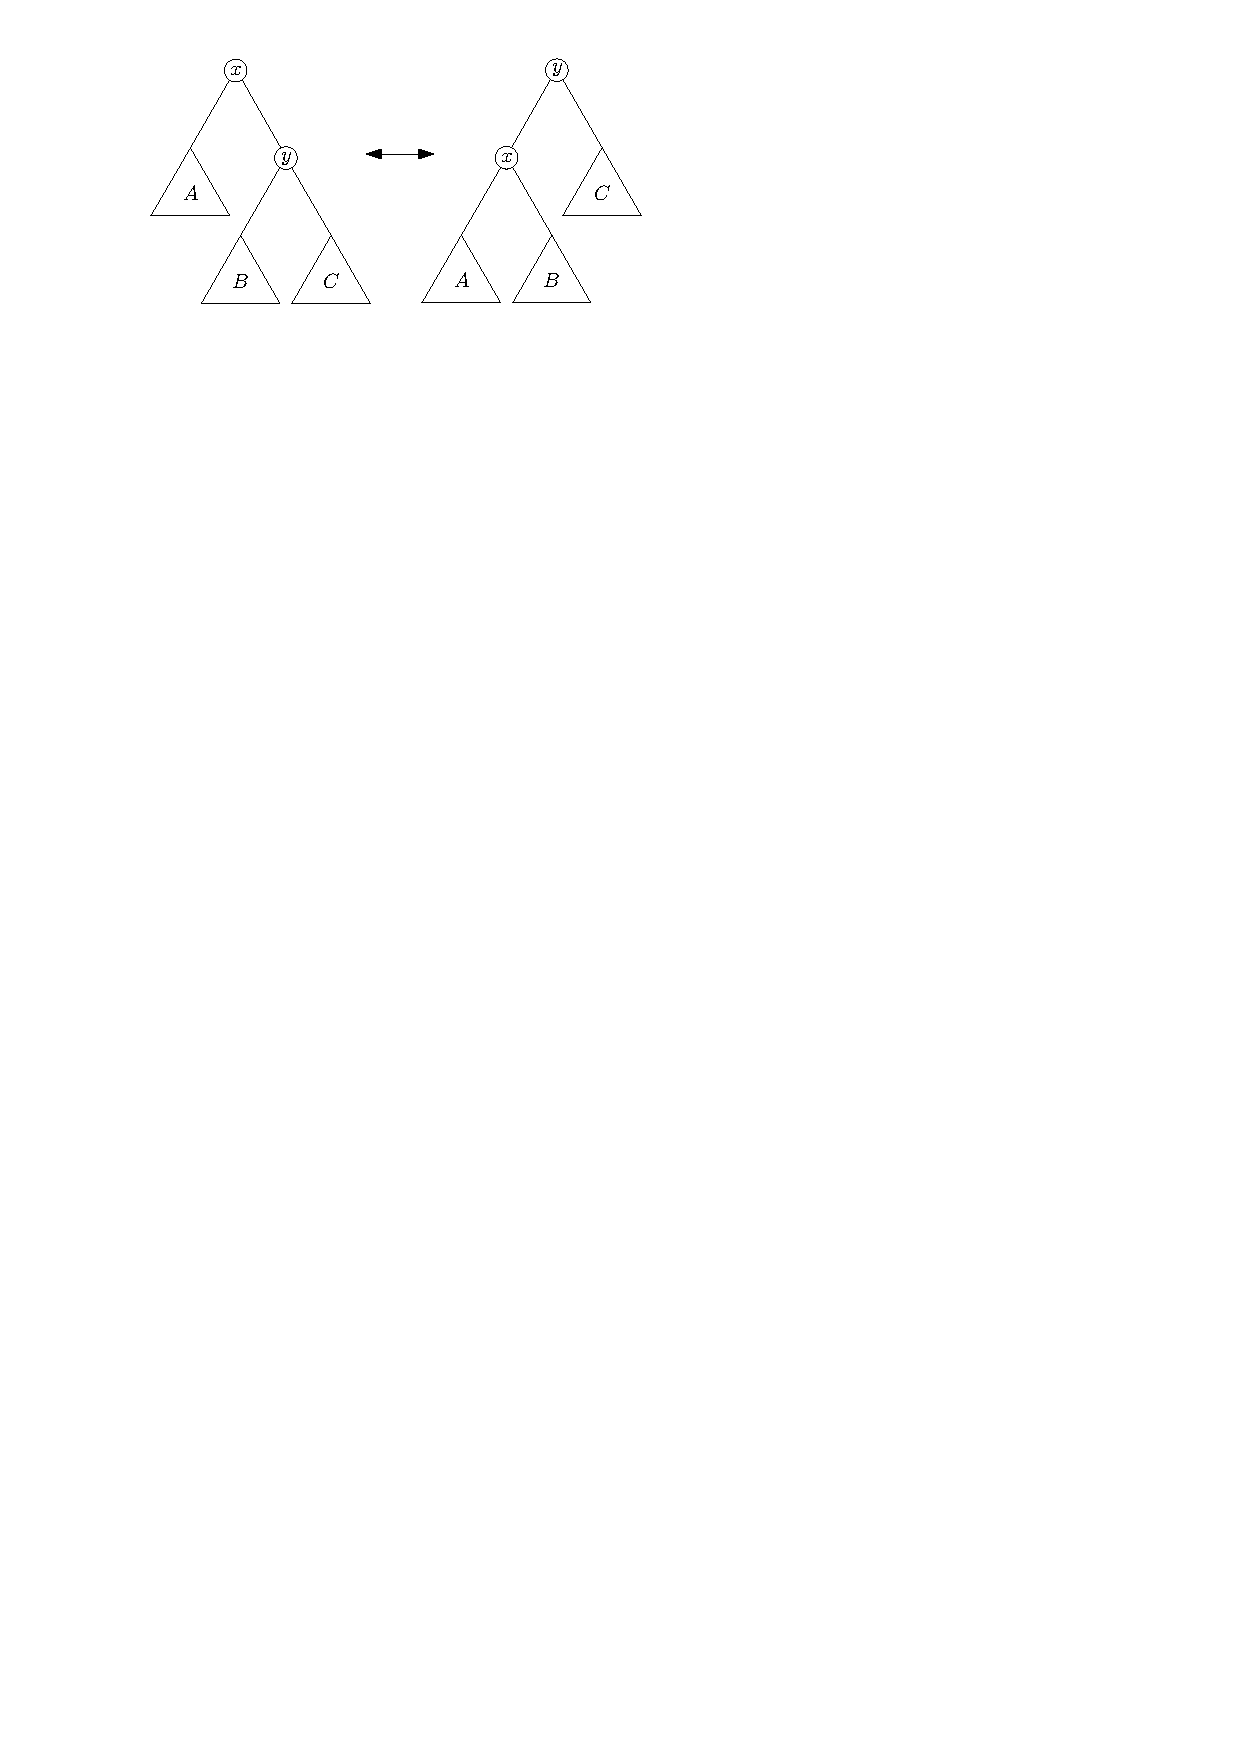
\includegraphics[width=.99\linewidth]{../img/single_rotation}
\end{subfigure}&

\begin{subfigure}{0.45\textwidth}
  \centering
  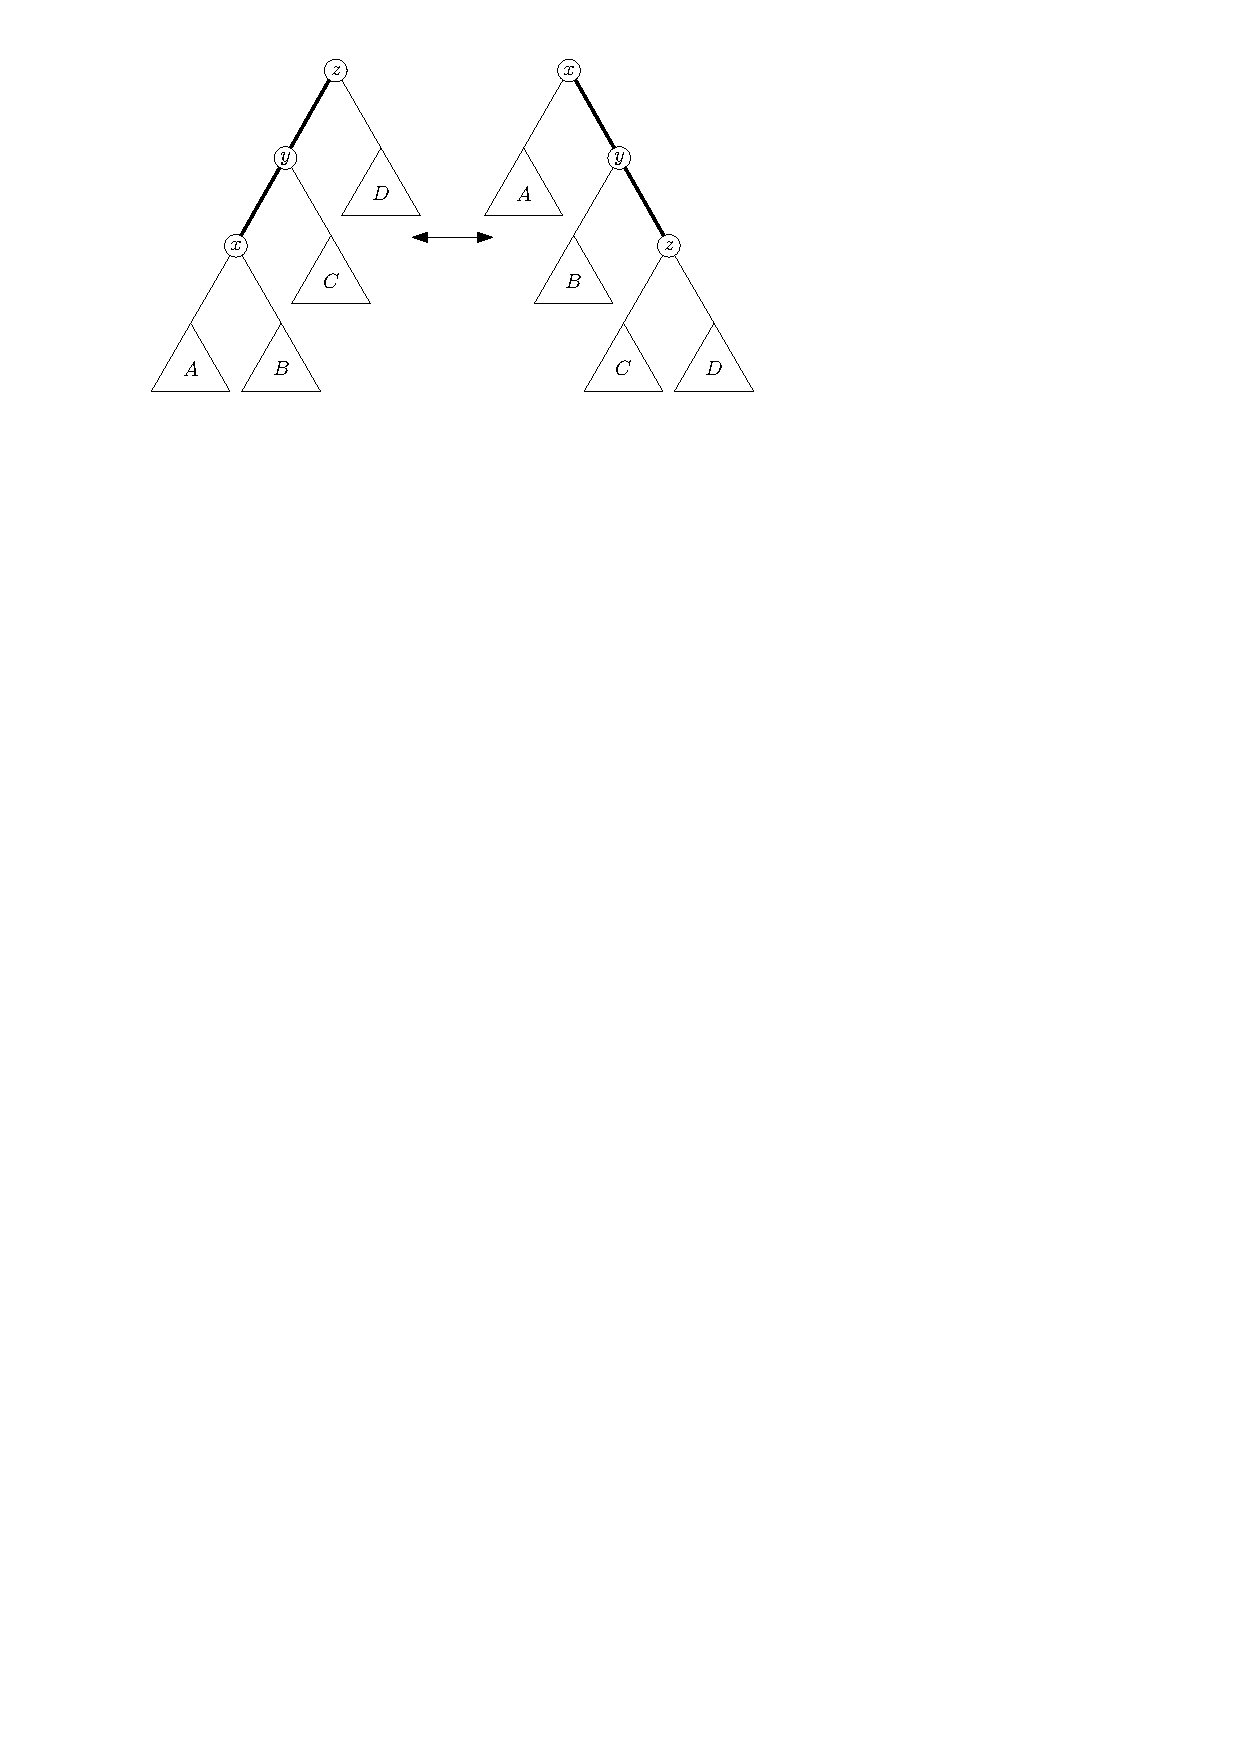
\includegraphics[width=.99\linewidth]{../img/zigzig_rotation}
\end{subfigure}\\

\noalign{\bigskip}
(a) Jednoduchá rotace hrany $xy$. 
&
(b) Zig-zig rotace.\\
\noalign{\bigskip}

\multicolumn{2}{c}{
\begin{subfigure}{0.9\textwidth}
  \centering
  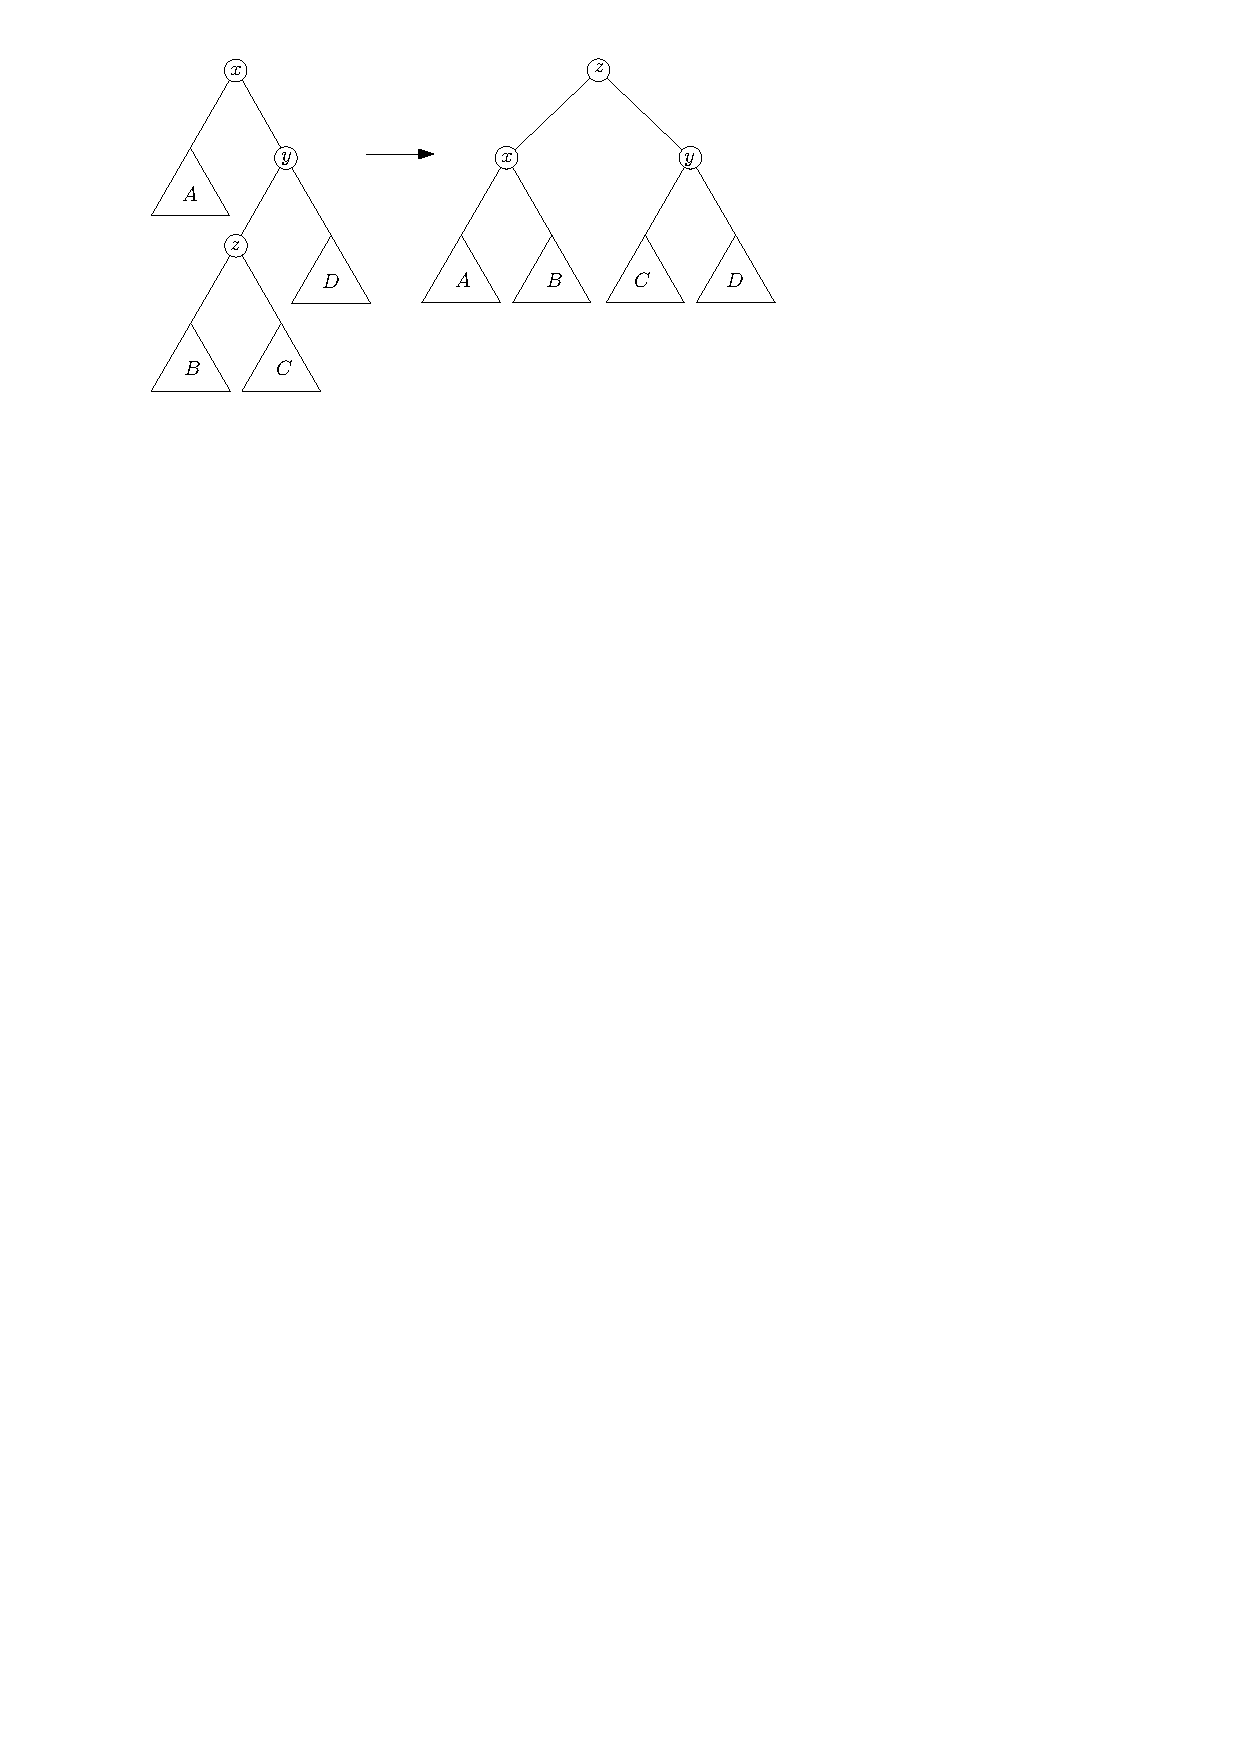
\includegraphics[width=.65\linewidth]{../img/zigzag_rotation}
\end{subfigure}}\\
\noalign{\bigskip}
\multicolumn{2}{c}{
  (c) Zig-zag rotace. Tato rotace jako jediná není symetrická.
}
\end{tabular} 
\caption{Jednoduchá, zig-zag a zig-zig rotace.} 

\label{obr:rotace} 
 
\end{figure}

\begin{definice}
Mějme vrchol binárního vyhledávacího stromu $u$ a jeho (bez újmy na obecnosti levého) syna $v$. Dále si
označme $p$ rodiče vrcholu $u$, $A$ a $B$ popořadě levý a pravý podstrom $v$ a
$C$ pravý podstrom $u$. Pak \emph{(jednoduchá) rotace hrany $uv$} je krok,
při němž nastavíme vrchol $v$ jako syna $p$ (na stejné straně, kde byl původně
vrchol $u$), vrchol $u$ jako pravého syna $v$ a podstrom $B$ jako levý podstrom
$u$. Podstromy $A$ a $C$ zůstanou připojené k~vrcholům $v$ a $u$ tak, jak byly.

Dále mějme vrchol $u$, jeho (bez újmy na obecnosti levého) syna $v$ a syna
vrcholu $v$, kterého si označíme $w$. Potom, pokud $w$ je pravý syn, můžeme
provést \emph{dvojitou rotaci hran $wv$ a $vu$ typu zig-zag}, která probíhá tak,
že nejprve zrotujeme hranu $wv$, a potom hranu $vu$. Pokud je $w$ levý syn,
můžeme provést \emph{dvojitou rotaci hran $wv$ a $vu$ typu zig-zig}, která
probíhá tak, že nejprve zrotujeme hranu $vu$ a potom hranu $wv$.
\end{definice}

Rotace hrany se může jevit jako zvláštní operace. Téměř všechny vyvažovací algoritmy (a úplně všechny, o~kterých zde budeme mluvit) ale využívají k~vyvažování právě rotace, protože se jedná o~poměrně jednoduchou a překvapivě silnou operaci, která zachovává uspořádání.

Dvojité rotace typu zig-zig budeme používat později v~této kapitole. Pro teď
si vystačíme s~jednoduchými rotacemi a dvojitými rotacemi typu zig-zag,
proto budeme-li mluvit o~dvojitých rotacích, budeme tím mít na mysli právě typ
zig-zag.

\subsection{AVL stromy}

AVL strom poprvé představili \citet{AVL}. Jedná se o~typ vyvažovaného stromu.
V~AVL stromu platí, že hloubka pravého a levého podstromu\footnote{Pravým, resp. levým podstromem vrcholu myslíme podstrom pravého, resp. levého syna tohoto vrcholu.} každého vrcholu se liší
nejvýše o~jedna. To znamená, že pokud $D(n)$ označíme minimální počet vrcholů
ve stromu hloubky $n$, dostáváme, že $D(0)=0$, $D(1)=1$ a
$D(i)=1+D(i-1)+D(i-2)$ pro každé $i$ větší než jedna. Pokud vyřešíme tuto
rekurenci, zjistíme, že $D(i)=\log_\varphi(i) + \o(1)$, kde $\varphi = 1.618\dots$ je zlatý
řez.

V~každém vrcholu si budeme pamatovat navíc informaci o~vyvážení daného vrcholu.
Tato informace může nabývat tří možných hodnot -- příslušný vrchol může být buď
\emph{vyvážený} (oba jeho podstromy jsou stejně hluboké), nebo \emph{nakloněný
doprava}, (jeho pravý podstrom je o~jedna hlubší než levý), nebo
\emph{nakloněný doleva}\footnote{Vystačili bychom si i s~jediným bitem, který by udával, zda je podstrom daného vrcholu hlubší než podstrom jeho sourozence.}.


\begin{figure}[h!]

\begin{subfigure}{0.9\textwidth}
  \centering
  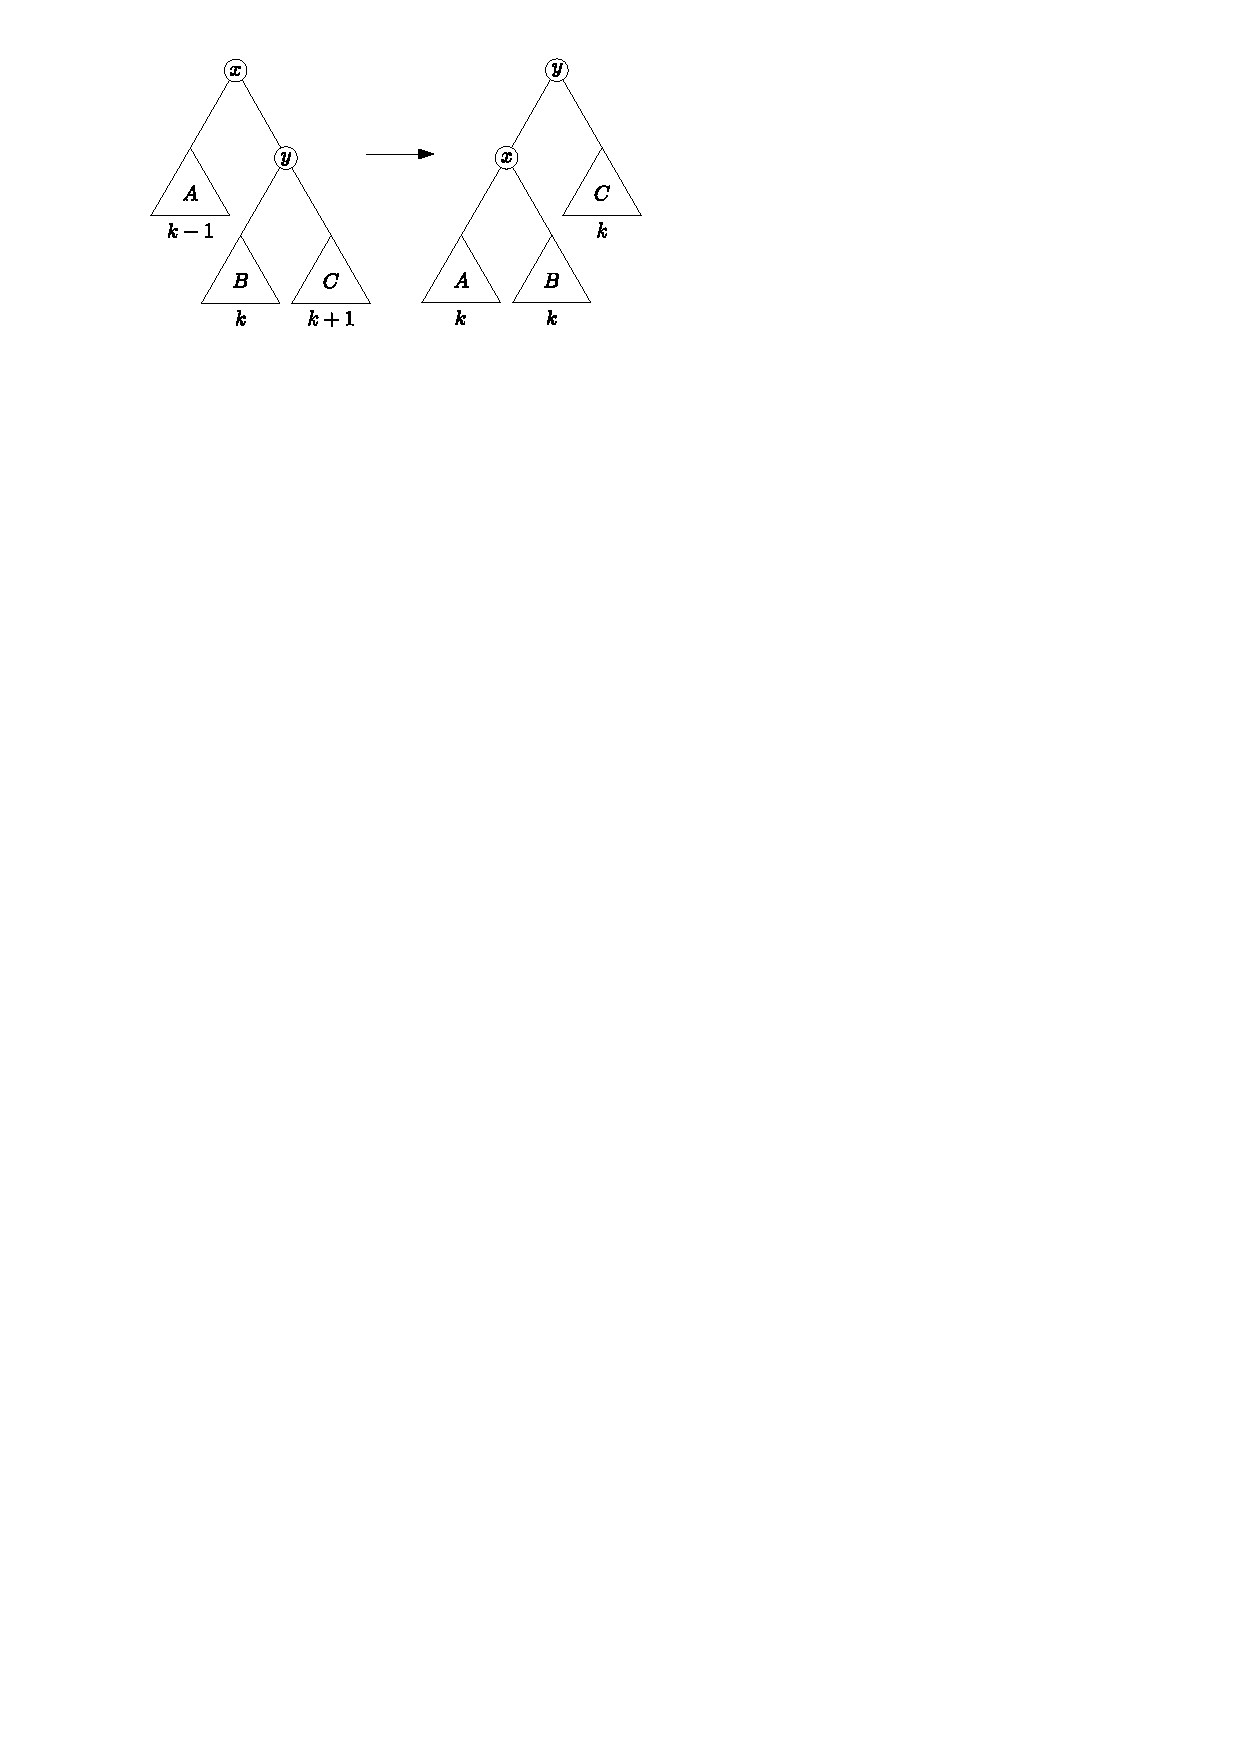
\includegraphics[width=.65\linewidth]{../img/single_rotation_avl}
\end{subfigure}
\vskip 1cm
\begin{subfigure}{0.9\textwidth}
  \centering
  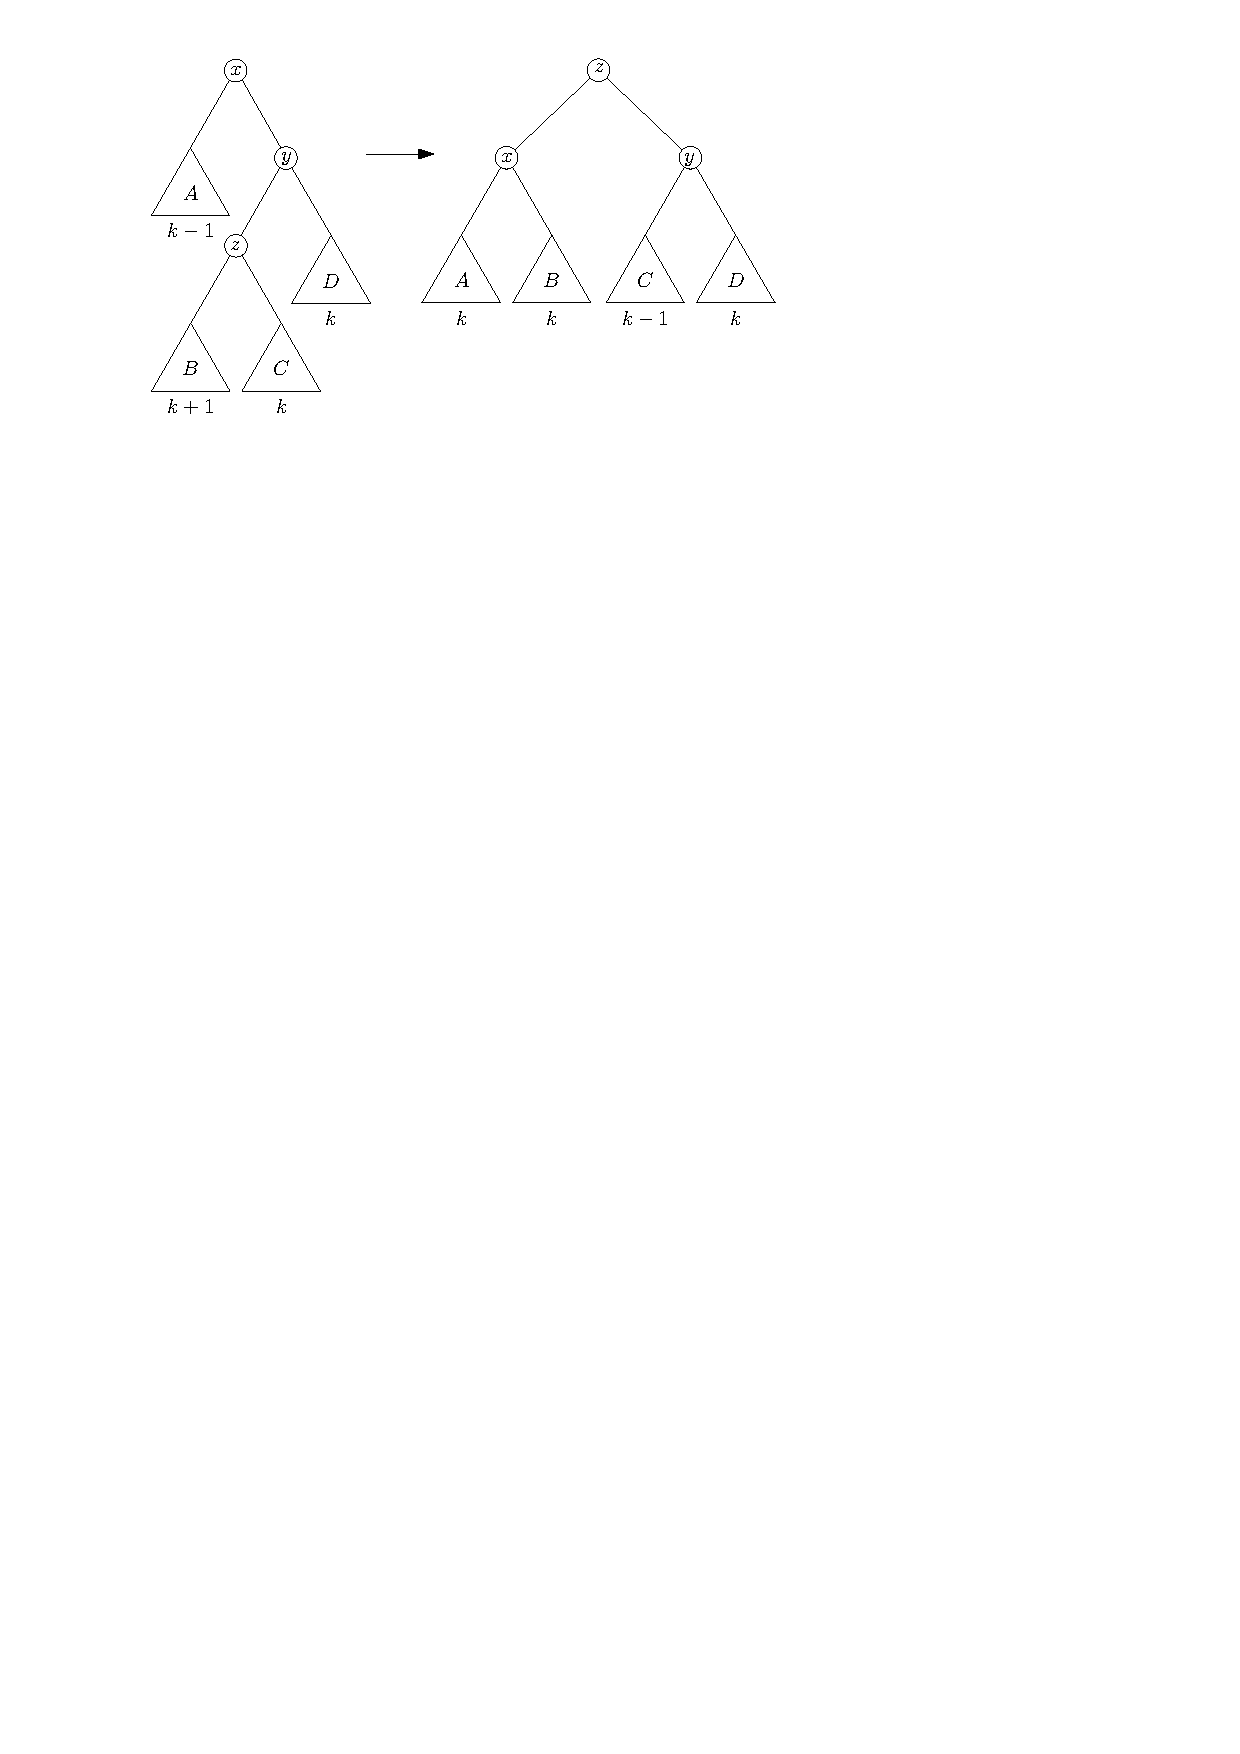
\includegraphics[width=.65\linewidth]{../img/zigzag_rotation_avl}
\end{subfigure}
\caption{Použití jednoduché a zig-zag rotace k~vyvážení AVL stromu.} 

\label{obr:rotace_avl} 
 
\end{figure}



Vyhledání prvku probíhá stejně, jako v~nevyvažovaném binárním vyhledávacím stromu. 
Vkládání je ale trochu komplikovanější. Při připojení nového listu je potřeba
jeho rodiči změnit vyvážení. Byl-li vyvážený (tj. byl to list), nově bude
nakloněný za novým vrcholem. Byl-li nakloněný od nového vrcholu, bude nově
vyvážený. V~prvním případě navíc vzrostla celková hloubka podstromu tohoto
vrcholu, je tedy potřeba změnu vyvážení propagovat výše do stromu. Kromě
předchozích dvou případů  může při další propagaci nastat ještě jeden jiný,
totiž že byl vrchol už původně nakloněný směrem, ze kterého propagujeme. To
znamená, že po přidání nového vrcholu již neplatí invariant AVL stromu a musíme
provést buď jednoduchou, nebo dvojitou rotaci hrany, abychom situaci napravili.

Nechť $x$ je nejhlubším vrcholem ve stromu, který po vložení vrcholu $v$ nesplňuje AVL invariant. Hloubku jeho podstromu před vložením $v$ si označíme $k$. Nechť byl bez újmy na obecnosti vložen vrchol do podstromu jeho pravého syna $y$. Pak je nutné rozebrat následující případy:
\begin{itemize}
\item Nový vrchol byl vložen do pravého podstromu vrcholu $y$ (první případ na
obrázku \ref{obr:rotace_avl}). Potom lze jednoznačně dopočítat hloubky
ostatních relevantních vrcholů (na obrázku pod podstromy; vždy počítáno vůči
kořenu nakreslené části stromu) na základě toho, že víme, že:
\begin{itemize}
\item Vrchol $x$ musí porušovat AVL
invariant, \item ostatní vrcholy ho musí splňovat, \item před vložením nového vrcholu
musely AVL invariant splňovat všechny vrcholy, \item hloubka podstromu $x$ musela
být $k$. 
\end{itemize}
Pak můžeme AVL invariant opravit jednoduchou rotací.  

\item Nový
vrchol byl vložen do levého podstromu $y$. Potom musíme provést
dvojitou rotaci. Jednu z~možných kombinací hloubek jednotlivých podstromů v~takovém případě zobrazuje
druhý případ na obrázku \ref{obr:rotace_avl}. Další možnost, kterou však není potřeba v~kódu
rozlišovat a vyřešíme ji úplně stejně, spočívá v~prohození hloubek podstromů
$B$ a $C$ z~tohoto obrázku.  
\end{itemize}

Provedením rotace však zařídíme, že se celý podstrom rotovaného vrcholu o~jedna
sníží. To znamená, že bude mít stejnou výšku jako před \ope{Insert}em a změnu tedy
není potřeba dále propagovat. Nabízí se otázka, když vyvažováním vždy
zajistíme, že se hloubka stromu nezmění, jak je možné, že do něj můžeme
postupně vložit libovolně mnoho vrcholů? Je to tím, že celková hloubka stromu
se může změnit právě při takových \ope{Insert}ech, které nezpůsobí žádnou
rotaci hrany.

Operaci \ope{Delete} zde podobně detailně probírat nebudeme, podotkneme ale, že na rozdíl od operace \ope{Insert} může být nutné až řádově logaritmicky mnoho rotací vůči vůči počtu vrcholů ve stromu (tj. lineárně mnoho vůči hloubce stromu). Kdybychom strom nejprve postavili posloupností operací \ope{Insert} a poté vymazali všechny vrcholy posloupností operací \ope{Delete}, mohli bychom ukázat, že provedeme amortizovaně konstantně mnoho rotací na operaci. Pokud však operace \ope{Insert} a \ope{Delete} nevhodně proložíme, může se stát, že budeme potřebovat až logaritmicky mnoho rotací na operaci.



\subsection{Červenočerný strom}\label{sec:RB}

Červenočerný strom odvodili z~2-4 stromů \citet{redblack}. Pro popis
červenočerného stromu se nám bude hodit alternativní pohled na binární stromy.
Představíme si, že na každé místo ve stromu, kde některému vrcholu chybí pravý nebo levý syn, přidáme jeden list.
Tím dostaneme strom, v~němž bude každý vrchol mít buď právě dva, nebo
žádného potomka. Vrcholy, které nemají žádného potomka, neobsahují žádný klíč
ani jiná data. V~programu tedy mohou být reprezentovány například nulovými
ukazateli. Těmto vrcholům budeme říkat \emph{vnější} nebo také \emph{externí}
vrcholy. Rozmyslíme si, že externích vrcholů je ve stromu s~$n$ neexterními
vrcholy $n+1$ a každý z~nich odpovídá jednomu intervalu mezi dvěma po sobě
jdoucími hodnotami ve stromu (nebo intervalu mezi jednou z~krajních hodnot a
plus nebo mínus nekonečnem).

Nyní již máme veškerou terminologii potřebnou k~tomu, abychom mohli přistoupit k~definici. Červenočerný strom je vyvažovaný binární strom, který dále splňuje následující invarianty:

\begin{enumerate}
\item Každý vrchol má buď červenou, nebo černou barvu.
\item Všechny externí vrcholy považujeme za černé.
\item Na každé cestě z~kořene do externího vrcholu musí být stejný počet černých vrcholů.
\item Každý červený vrchol má oba potomky černé.
\end{enumerate}

Některé zdroje dále uvádí, že kořen musí být černý, to však není problém
kdykoli zařídit -- máme-li korektní červenočerný strom s~červeným kořenem,
můžeme kořen přebarvit na černo a všechny invarianty zůstanou splněny. Pokud
však budeme černou barvu kořene požadovat, bude ve stromu lépe vidět souvislost
s~původními 2-4 stromy. V~takovém případě si můžeme všimnout, že pokud
zkontrahujeme všechny hrany mezi červeným synem černého otce, dostaneme strom,
ve kterém má každý vrchol kromě listů mezi dvěma a čtyřmi potomky a ve kterém
jsou všechny cesty z~kořene do listu stejně dlouhé.

Nyní se pokusíme odhadnout minimální počet vrcholů ve stromu hloubky
$n$. Tento minimální počet si označíme D(n). Strom s~minimálním počtem vrcholů při dané hloubce vypadá tak, že obsahuje
jednu cestu, na níž se střídají červené a černé vrcholy. Na každý její vrchol
dále pověsíme dokonale vyvážený strom tvořený pouze černými vrcholy o~hloubce
určené tak, aby byly splněny invarianty. To znamená, že jeden z~podstromů
kořene je strom s~minimálním počtem vrcholů při hloubce o~jedna menší a druhý
je dokonale vyvážený strom. Kdybychom se pokusili $D(n)$ vyjádřit pouze pomocí
$D(n-1)$, muselo by se nám ve vzorci objevit zaokrouhlování ve formě dolní celé
části. Abychom se zaokrouhlování vyhnuli, vyjádříme $D(n)$ pomocí $D(n-2)$.

$D(n)$ můžeme vyjádřit\footnote{V následujícím výpočtu nebereme v~úvahu externí vrcholy. Kdybychom je v~úvahu brali, přesné vzorce by vypadaly trochu jinak, ale v~závěru by se změna schovala v~$\o$-notaci.} jako $D(1)=1$, $D(2) = 2$, $D(2i) = D(2i-2) + 2 \cdot
(2^{i - 1} - 1) + 2$, $D(2i + 1) = D(2i - 1) + 2^{i-1}-1 + 2^i-1 + 2$. Z~toho
po zjednodušení a vyřešení dostáváme, že $D(i)\in\Theta(2^{i/2})$, tedy nejvyšší
možná hloubka s~daným počtem vrcholů je $H(n) = \log_{\sqrt 2} n + \o(1)$.
Protože  $\sqrt 2 < \varphi$, je hloubka červenočerného stromu v~nejhorším
případě větší než hloubka AVL stromu v~nejhorším případě při stejném počtu
vrcholů.

Průběh operací \ope{Insert} a \ope{Delete} zde nebudeme probírat, protože obsahují velké
množství speciálních případů, které by bylo potřeba popsat. Připojíme ale
dvě poznámky. První z~nich je, že výhodou červenočerných stromů oproti AVL
stromům je vždy pouze konstantně mnoho změn struktury stromu při operaci. Dále je zde
vhodné zmínit velice příbuznou struktura, tzv.
\emph{right-leaning červenočerný strom}, který představil \citet{rightleaning}.
V~tomto stromu oproti červenočernému stromu navíc platí, že pokud má vrchol právě jednoho červeného syna,
musí to být pravý syn. Tím sice může mírně vzrůst celkový počet rotací
k~vyvážení struktury, ale výrazně se sníží počet případů, které je třeba při
vyvažování řešit, a strom se tak stane implementačně výrazně jednodušším. V~této
práci dále pokračoval \citet{leftleaning}, který dále zakázal vrcholy, jejichž
oba synové by byli červení. V~této úpravě pak lze naimplementovat operaci
\ope{Insert} na pouhých 33 řádcích kódu v~jazyce Java.    

Červenočerné stromy ale dále umí dvě operace, jež zde představíme, protože
jich využívají datové struktury, které budeme popisovat později v~této práci. Bude se jednat o~operace \emph{\ope{Join}} a \emph{\ope{Split}}.
Před jejich popisem budeme ale potřebovat zavést ještě dva nové pojmy.

\begin{definice}
Mějme červenočerný strom $S$. Pak počet černých vrcholů na cestě mezi kořenem a (libovolným) externím vrcholem $S$ (nepočítaje koncové vrcholy této cesty) nazveme \emph{černou výškou} stromu $S$. Značit ji budeme $H'(S)$.
\end{definice}


\begin{definice}
Mějme libovolný neprázdný binární vyhledávací strom $S$ a jeho vrchol $u$, resp. $v$, odpovídající minimálnímu, resp. maximálnímu prvku v~něm. Pak cestu z~kořene do $u$, resp. $v$ nazveme \emph{levou}, resp. \emph{pravou páteří} stromu $S$.
\end{definice}

Operace \ope{Join} má na vstupu dva červenočerné
stromy $A$, $B$ a jeden další prvek univerza $x$. Pro tyto stromy musí platit,
že hodnoty všech prvků ve stromu $A$ jsou menší než $x$ a hodnoty všech prvků
ve stromu $B$ jsou větší než $x$. Na výstupu operace \ope{Join} máme jeden strom
obsahující všechny prvky, které obsahoval strom $A$, strom $B$, a prvek $x$. Za
předpokladu, že předem známe černou výšku stromů $A$
a $B$ $H'(A)$ a $H'(B)$, operaci \ope{Join} zvládneme v~čase $\Theta(1+|H'(A) -
H'(B)|)$.

Při provádění operace \ope{Join} budeme postupovat následovně:

\begin{enumerate}
\item Pokud $H'(A) = H'(B)$, pak můžeme vytvořit nový černý vrchol s~hodnotou $x$, jako jeho levého a pravého syna nastavit kořeny stromů $A$ a $B$ a vrátit ho jako kořen nového stromu.
\item Jinak bez újmy na obecnosti předpokládejme, že $H'(A)<H'(B)$. Potom můžeme jít po pravé páteři stromu $A$, dokud nenalezneme vrchol $v$ takový, že černá výška jeho podstromu je $H'(B)$. Vytvoříme nový červený vrchol $u$ s~hodnotou $x$ a vložíme ho do stromu na místo vrcholu $v$. Vrchol $v$ připojíme pod $u$ jako levého syna a kořen stromu $B$ jako pravého syna. Mohlo se stát, že jsme právě rozbili invariant červenočerného stromu. Jeho platnost tedy obnovíme podobným postupem jako při normálním \ope{Insert}u.
\end{enumerate}

Druhou operací je operace \ope{Split}. Operace \ope{Split} dostane na vstupu
strom\footnote{Z popisu operace \ope{Split} vyplyne, že není specifická pro
červenočerné stromy. Tuto operaci můžeme provést s~libovolným typem binárního
vyhledávacího stromu, který podporuje operace \ope{Delete} a \ope{Join}. Pouze
analýza časové složitosti bude specifická pro červenočerné stromy.} $S$ a $x\in
\mathcal U$. Na výstupu má dva stromy $A$, $B$ takové, že všechny prvky ve
stromu $A$ budou menší než $x$, a prvky ve stromu $B$ jsou větší než $x$.
Stromy $A$ a $B$ navíc obsahují dohromady tytéž prvky jako strom $S$ (kromě
prvku $x$, pokud tento prvek byl ve stromu $S$). Operace \ope{Split} proběhne
na červenočerném stromu v~čase $\o(\log n)$. Postup bude následující:

\begin{enumerate}

\item Vyhledáme ve stromu $S$ prvek $x$. Pokud si v~naší implementaci
červenočerného stromu nepamatujeme u~každého vrcholu černou výšku jeho
podstromu, při cestě dolů budeme tyto černé výšky počítat. To můžeme udělat
například tak, že si ke každému vrcholu poznamenáme, kolik černých vrcholů je
na cestě mezi ním a kořenem (kořen včetně, vrchol sám nevčetně). Poté spočítáme
černou výšku celého stromu (pokud $x$ ve stromu není, stačí spočítat počet
černých vrcholů na cestě mezi kořenem a externím vrcholem, na jehož místo
bychom $x$ vkládali. Jinak pokračujeme stromem dolů až k~libovolnému externímu
listu). Černá výška podstromů jednotlivých vrcholů je pak rovna rozdílu mezi číslem,
které jsme si k~nim poznamenali, a černou výškou původního
stromu\footnote{Černou výšku celého stromu ve skutečnosti ani počítat nemusíme.
Pro \ope{Join} ve skutečnosti nepotřebujeme znát černé výšky, stačí nám pouze umět
v~konstantním čase určit rozdíl černých výšek dvou stromů, což lze již ze
zapamatovaných čísel.}.

\item Na cestě, kterou při vyhledání procházíme, odstraňujeme všechny hrany.
Vrcholy si roztřídíme do dvou seznamů podle toho, zda jsou větší nebo menší než
$x$. V~seznamech udržujeme pořadí, v~jakém jsme vrcholy na cestě našli --
seznamy jsou setříděné podle černých výšek podstromů, které zůstaly viset na
vrcholech. Pokud bylo $x$ ve stromu, odstraníme ho a na konec našich seznamů
připojíme vždy příslušného syna $x$.

\item Nyní tedy máme dva seznamy vrcholů, v~nichž na každém z~vrcholů visí
právě jeden syn. Podstrom tohoto syna je vždy validní červenočerný strom, a
navíc známe jeho černou výšku. Výjimkou může být vždy poslední vrchol v~seznamu
-- ten může mít oba syny, v~kterémžto případě je již on sám kořenem korektního
červenočerného stromu. Navíc platí, že oba seznamy jsou setříděny podle černých
výšek stromů (tyto černé výšky nemusí být po dvou různé). Dále platí, že
v~seznamu prvků větších než $x$ je hodnota každého vrcholu menší než hodnota všech
prvků v~jeho zbývajícím (pravém) podstromu. Současně je ale větší než hodnota všech prvků
(a jejich zbývajících podstromů), které jsou v~seznamu dále než daný vrchol (protože se
původně jednalo o~části jeho levého podstromu). Nyní tedy pro každý seznam
zvlášť:
\begin{itemize}

\item Pokud poslední prvek seznamu není kořenem korektního červenočerného
stromu, udělej z~něj korektní červenočerný strom. To znamená, že vezmeme
červenočerný strom, který visí na prvku seznamu, a prvek, na kterém tento strom původně
visel, do něj vložíme standardní operací \ope{Insert}.

\item Všechny prvky seznamu spojíme operací \ope{Join}. Budeme postupovat od
konce, a to vždy tak, že vezmeme poslední prvek seznamu, což je validní
červenočerný strom, syna předposledního prvku, což je také červenočerný strom,
a hodnotu předposledního prvku (která je mezi hodnotami obsaženými ve dvou zmíněných stromech), a aplikujeme na tyto dva stromy
a tento prvek operaci \ope{Join}. Výsledný strom připojíme opět na konec
seznamu. 

\end{itemize}
\end{enumerate}

Úvodní hledání $x$ zvládneme v~čase $\o(\log n)$. Při slučování využijeme
toho, že stromy byly původně seřazeny podle černé výšky a spojování tuto výšku
změnilo nejvýše o~konstantu (uvědomíme si, že vždy nejvýše dva po sobě jdoucí
stromy mohly mít původně stejnou černou výšku, černé výšky tedy nemohou růst
příliš). Součet všech rozdílů černých výšek spojovaných stromů je tedy nejvýše
výška původního stromu plus jejich počet vynásobený vhodnou konstantou. Oba sčítance jsou
nejvýše $\o(\log n)$, celá operace \ope{Split} tedy proběhne v~čase $\o(\log
n)$.

\subsection{Rankově vyvažované stromy}

\citet{rankbalanced} vyšli z~myšlenek Guibase a Sedgewicka \citeyearpar{redblack}, kteří zobecnili
myšlenku červenočerných stromů, a představili nový způsob uvažování
o~vyvažovaných stromech. Každému vrcholu přiřadili celočíselný rank, přičemž
externí vrcholy mají rank $-1$ a rank ostatních vrcholů je nezáporný. Různým
nastavením pravidel pro rozdíly ranků mezi vrcholem a jeho syny potom dostali
různé datové struktury. Abychom však o~těchto strukturách mohli snadno mluvit,
musíme nejprve zavést několik pojmů.

\begin{definice}
Řekneme, že vrchol binárního vyhledávacího stromu je \emph{$a$-syn}, pokud rozdíl jeho ranku a ranku jeho rodiče je právě $a$. O~vrcholu řekneme, že je \emph{$(a,b)$-vrcholem}, pokud jeho potomci jsou (ne nutně v~tomto pořadí) $a$-syn a $b$-syn.
\end{definice}

Všimneme si, že pokud si jako pravidlo zvolíme, že každý vrchol bude $(1,1)$
nebo $(1,2)$-vrchol, bude rank každého vrcholu roven právě délce nejdelší cesty
(počítané počtem hran) z~něj do listu v~jeho podstromu, a výsledný strom bude
AVL strom\footnote{Všimneme si, že v~tomto myšlenkovém rámci dává smysl, aby si každý vrchol pamatoval, zda je $1$-synem či $2$-synem. Pak dostáváme přesně AVL strom s~jediným bitem vyvažovací informace na vrchol, který jsme popsali v~poznámce pod čarou výše.}. Pokud si jako pravidlo zvolíme, že každý vrchol kromě kořene je
$1$-syn nebo $0$-syn a žádný $0$-syn není synem $0$-syna, dostaneme
červenočerný strom, v~němž $1$-synové odpovídají černým vrcholům (požadavek na
nezápornost ranků vrcholů zajišťuje, že všechny externí vrcholy jsou
$1$-synové).

Existuje ale ještě jiné pravidlo, kterým dostaneme červenočerné stromy. Pokud
povolíme $1$-syny a $2$-syny, dostáváme také červenočerné stromy. Nyní ovšem
černým vrcholům odpovídají nejen $2$-synové, ale i $1$-synové s~lichým rankem.
Takový strom určitě invariant červenočerného stromu splňuje -- máme-li dva
vrcholy spojené hranou se sudým rankem, je (minimálně) spodní z~nich 2-syn.
Naopak pokud máme libovolný červenočerný strom, můžeme každému vrcholu $v$, jehož
podstrom si označíme $S$, přiřadit rank $2\cdot H'(S)$, pokud je $v$ červený a
$2\cdot H'(S) + 1$ pokud je černý.

Toto pravidlo lze formulovat také tak, že každý vrchol je buď $(1,1)$, $(1,2)$ nebo $(2,2)$-vrchol. Toto pravidlo vypadá podobně jako AVL pravidlo. Mohli bychom se tedy ptát, zda neexistuje nějaké pravidlo, které by bylo restriktivnější než pravidlo červenočerných stromů, ale volnější než pravidlo AVL stromů, které by nám umožnilo spojit výhody obou těchto stromů. Připomeneme, že výhodou AVL stromu je o~něco menší hloubka nejhlubšího vrcholu v~nejhorším případě, výhodou červenočerných stromů je garance nejvýše $\o(1)$ změn struktury na operaci. 

Toho skutečně lze dosáhnout, a to pomocí následujících dvou pravidel:
\begin{enumerate}
\item Všechny listy (tj. vrcholy, jejichž oba synové jsou externí) jsou $(1,1)$-vrcholy.
\item Všechny ostatní vrcholy jsou buď $(1,1)$, $(1,2)$ nebo $(2,2)$-vrcholy.
\end{enumerate}

S~touto sadou pravidel navíc s~(přímočarými) \ope{Insert} a \ope{Delete} algoritmy, které \citet{rankbalanced} popsali, dostáváme \emph{Weak AVL} strom, který má následující vlastnosti:

\begin{itemize}
\item Při \ope{Insert}ech nevznikají $(2,2)$-vrcholy -- pokud vrcholy pouze vkládáme, máme AVL strom.
\item Nastane pouze $\o(1)$ změn struktury stromu na operaci v~nejhorším případě.
\item Nastane pouze amortizovaně $\o(1)$ změn ranku na operaci. Navíc počet změn ranku vrcholu ranku $k$ je amortizovaně $\o(\varphi^{-k})$ na operaci.
\item Pokud $n$ je počet vrcholů stromu a $m$ je počet operací \ope{Insert} za celou dobu života struktury, pak hloubka stromu je nejvýše $\min(\log_{\varphi} m, \log_{\sqrt2} n) + \o(1).$ Z~toho vyplývá, že pokud $m\in\Theta(n)$, tj. pokud máme ve stromu alespoň řádově stejně prvků, kolik jsme jich smazali, bude hloubka Weak AVL stromu v~nejhorším případě až na aditivní konstantu stejná jako hloubka AVL stromu na stejném počtu prvků v~nejhorším případě.
\item Weak AVL strom lze rebalancovat nejen zdola nahoru, ale i preventivně shora dolů, což může být výhodné při paralelní práci se stromem. Pak ale ostatní zde uvedené body neplatí.
\end{itemize}



\section{Výpočetní model}\label{sec:model}
Chceme-li mluvit o~optimálním stromu, musíme nejprve specifikovat, co přesně
budeme za binární vyhledávací strom považovat. Pro zjednodušení se opět vrátíme
ke stromům nad pevnou množinou klíčů. Nebudeme tedy podporovat operace \ope{Insert} a \ope{Delete}\footnote{Budeme předpokládat, že strom již stavíme nad neprázdnou množinou klíčů.}.
Definici, kterou zde
představíme, používali implicitně už \citet{splay}, formalizoval ji však až
\citet{tango}.


\begin{definice}
Mějme \emph{přístupovou posloupnost} $S$ $x_1$,$x_2$,\dots,$x_m$, kde $\forall i \in
\mathbb N, i\leq m$ platí $x_i\in M$. Pak \emph{přístupový algoritmus
binárního vyhledávacího stromu} je algoritmus, který postupně provede přístupy
ke vrcholům s~klíči $x_1, x_2,\dots,x_m$.

Přístup probíhá tak, že algoritmus smí mít vždy právě jeden ukazatel na vrchol
stromu, který na počátku každého přístupu ukazuje na kořen stromu. Dále
v~každém kroku smí provést právě jeden z~kroků tak, jak byly popsány v~úvodu této kapitoly, případně rotaci hrany mezi aktuálním vrcholem a jeho rodičem. 

Řekneme, že časem běhu algoritmu je počet těchto kroků, které algoritmus za sekvenci
přístupů provede, plus jedna\footnote{Čas strávený výpočtem toho, jaký krok se má provést, zanedbáme.}. O~vrcholu stromu řekneme, že jsme se ho při daném
přístupu \emph{dotkli}, pokud na něj někdy během tohoto přístupu ukazoval
ukazatel algoritmu.  \end{definice}

Takovému přístupovému algoritmu se někdy také říká \emph{offline přístupový
algoritmus}. V~praxi ale potřebujeme přístupy provádět online.

\begin{definice}
\emph{Online přístupový algoritmus} je takový přístupový algoritmus, jehož
rozhodnutí během $i$-tého přístupu nijak neovlivňují hodnoty $x_j$ z~přístupové
posloupnosti pro $j>i$. Na druhou stranu si tento algoritmus smí v~každém
vrcholu uložit až $\mathcal O(1)$ slov paměti informací (nikoli však ukazatele
na vrcholy).
\end{definice}

Všimneme si, že běžné algoritmy binárních vyhledávacích stromů tuto definici
splňují -- například červenočerné a AVL stromy potřebují v~každém vrcholu
jediný bit informace, splay strom se obejde zcela bez dalších informací.

Pro danou přístupovou sekvenci $S$ existuje přístupový algoritmus, který ji
vykoná optimálně, tedy v~nejkratším čase ze všech možných algoritmů. Tento
počet kroků označíme $\opt(S)$. Zde předpokládáme, že je strom na začátku
v~nejlepší možné konfiguraci. Tím však nesnížíme čas potřebný na přístupy o~více
než aditivní $\mathcal O(n)$, protože z~libovolného BVS je možné pomocí
$\mathcal O(n)$ rotací vytvořit libovolný jiný (nad toutéž množinou klíčů).
Proto budeme dále zkoumat pouze přístupové posloupnosti $S$ takové, že $m \in
\Omega(n)$. Vzhledem k~tomu, že nahlédneme, že $\opt(S)\geq m$, je aditivní
faktor $\o(n)$ asymptoticky zanedbatelný. 


\begin{definice}
O~přístupovém algoritmu řekneme, že je \emph{$f(n)$-kompetitivní}, pokud libovolnou
posloupnost přístupů $X$ nad univerzem velikosti $n$ vykoná v~čase $
\o(f(n))\cdot\opt(X)$. O~online přístupovém algoritmu řekneme, že je
\emph{dynamicky optimální}, pokud je $\mathcal O(1)$-kompetitivní.
\end{definice}

Předtím, než si popíšeme některé konkrétní stromy, už pouze podotkneme, že
existence dynamicky optimálního algoritmu je otevřeným problémem. Na druhou
stranu například o~splay stromech vyslovili \citet{splay} hypotézu, že jsou
dynamicky optimální.

\section{Splay stromy}

Splay strom představili \citet{splay}. Jedná se o~strom, který modifikuje svou
strukturu nejen při operacích \ope{Insert} a \ope{Delete}, ale i při
vyhledávání\footnote{Přestože splay strom vkládání i mazání podporuje, my se
nyní zabýváme modelem, kde stromy umí pouze vyhledávat. Proto budeme
předpokládat, že operaci \ope{Delete} nikdy nevykonáme a všechny operace
\ope{Insert} vykonáme před začátkem měření v~rámci inicializace struktury.}.
Splay strom podporuje operaci $\ope{Splay}(x)$, a všechny ostatní stromové
operace implementuje pomocí $\o(1)$ volání této operace.

Samotná operace $\ope{Splay}(x)$ se skládá ze dvou fází: nejprve standardním způsobem
vyhledáme vrchol stromu obsahující klíč $x$ a poté tento vrchol pomocí rotací
hran přesuneme do kořene. V~případě neúspěšného hledání přesuneme do kořene poslední navštívený vrchol. Někdy také operaci \ope{Splay} definujeme pouze jako přesun vrcholu rotacemi do kořene -- pak musíme dostat jako argument této operace rovnou ukazatel na vrchol.

Při přesouvání vrcholu do kořene postupujeme tak, že
pokud je vzdálenost aktuálního vrcholu od kořene stromu alespoň dva, použijeme
vždy dvojitou rotaci (v~závislosti na tom, zda jsou splayovaný vrchol a jeho
rodič synové na téže či různé straně, použijeme buď zig-zig rotaci, nebo zig-zag
rotaci). Pouze ve chvíli, kdy je splayovaný vrchol synem kořene, použijeme
jednoduchou rotaci. Tento postup má za následek, že hloubka splayovaného vrcholu se sníží na nulu, hloubka všech ostatních vrcholů, kterých se během splayování dotkneme, se sníží přinejmenším o~polovinu (až na aditivní konstantu) a hloubka vrcholů, kterých jsme se nedotkli, se zvýší maximálně o~konstantu.

Pomocí operace $\ope{Splay}(x)$ naimplementujeme ostatní stromové operace. Při
operaci \ope{Insert}(x) nejprve zavoláme $\ope{Splay}(x)$. Tím se dostane
následník nebo předchůdce $x$ do kořene. Potom můžeme vložit nový vrchol
obsahující $x$ mezi něj a jeho pravého nebo levého syna. Při operaci \ope{Delete} na
prvek zavoláme $\ope{Splay}$, poté ze stromu odstraníme kořen a dva vzniklé
stromy (jsou-li oba neprázdné)  spojíme dále popsanou operací \ope{Join}.
Operaci \ope{Join} tak, jak byla popsána v~kapitole \nameref{sec:RB}, můžeme
provést tak, že ve stromu, který bez újmy na obecnosti obsahuje menší prvky ze
dvou spojovaných stromů, zavoláme $\ope{Splay}(\infty)$. Tím dostaneme nejvyšší
prvek do kořene. Kořeni proto bude chybět pravý syn. Na jeho místo tedy můžeme
připojit druhý strom. Pokud máme v~rámci spojování prvek mezi hodnotami obou
stromů do stromu vložit, stačí ho prohlásit za nový kořen a jako syny mu
připojit kořeny původních stromů. \ope{Split} provedeme následovně:

\begin{enumerate}
\item $\ope{Split}(x)$ v~našem případě rozdělí strom na stromy s~hodnotou klíče větší než $x$, menší než $x$, případně nechá samostatně vrchol s~hodnotou $x$, pokud ve stromu byl. Začneme tedy zavoláním $\ope{Splay}(x)$.
\item Pokud byl vrchol s~klíčem $x$ nalezen, máme hotovo -- vrátíme samostatně kořen stromu a jeho jednotlivé podstromy jako výstup.
\item Jinak bez újmy na obecnosti nechť máme v~kořeni vrchol s~klíčem větším než $x$. Jedná se ale o~nejbližší větší klíč, proto můžeme odpojit jeho levého syna a oba takto vzniklé stromy vrátit jako výstup.
\end{enumerate}

Splay strom nám garantuje logaritmickou amortizovanou složitost operace
$\ope{Splay}$. V~některých situacích může však být i lineárně hluboký. Pokud
například přistoupíme ke všem prvkům v~rostoucím pořadí, bude mít strom tvar
cesty, kde každý vrchol (krom jediného listu) bude mít pouze levého syna. Pokud
poté zavoláme $\ope{Splay}$ na nejmenší prvek ve stromu, operace bude trvat lineárně
dlouho, avšak hloubku stromu zmenší o~polovinu.

Jak už jsme napsali výše, o~splay stromu byla vyslovena hypotéza, že je
dynamicky optimální, avšak pro obecnou přístupovou posloupnost pro něj nebylo
dokázáno nic silnějšího, než triviální $\log(n)$-kompetitivita. Pro některé
konkrétní přístupové sekvence byly však pro splay strom dokázány zajímavé
výsledky, které si představíme v~další kapitole.

\section{Meze optimality}

Definice optimality uvedená v~sekci \ref{sec:model} bohužel není příliš užitečná, protože není
znám algoritmus, který by efektivně spočítal chování optimálního binárního
vyhledávacího stromu. Proto různí autoři přišli s~různými odhady na $\opt(S)$.
My zde předvedeme několik horních odhadů a jeden dolní odhad. Začneme třemi
odhady, které představili \citet{splay}. Ti ve svém článku ukázali, že
všechny tři meze (až na aditivní člen závisející pouze na $n$) splay strom
splňuje. Proto musí platit i pro optimální strom. Proč můžeme pro optimální
stromy aditivní členy závisející pouze na $n$ vypustit, vysvětlíme v~této sekci později.

\begin{veta}[Static Optimality Bound]
Mějme přístupovou posloupnost $S$ délky $m$ nad množinou $[n]$, a nechť $q:[n]\rightarrow \mathbb N_0$ určuje počet výskytů každého prvku $[n]$ v~$S$. Potom $$\opt(S) \in \o\left(m + \sum_{i\in [n]}q(i)\log\frac m{q(i)}\right).$$
\end{veta}

Tento odhad splňuje i statický optimální strom popsaný v~sekci \nameref{sec:staticoptimality}. Proto také všem stromům, které tuto mez splňují, říkáme staticky optimální.  

\begin{veta}[Static Finger Bound]
Mějme přístupovou posloupnost $S$ délky $m$ nad množinou $[n]$ jejíž $i$-tý prvek si označíme $s_i$. Potom pro libovolné $f\in [m]$ platí $$\opt(S) \in \o\left(m + \sum_{i\in [m]} \log(1 + |f-s_i|) \right).$$
\end{veta}

Tento odhad jinými slovy říká, že strom musí umět rychle odpovídat na dotazy na
prvky blízko libovolného fixního prvku. Tuto mez původně představili v~silnější
verzi \citet{fingersearchtree} v~článku o~\emph{prstovém vyhledávacím stromu}. To je
struktura, která umožňuje udržovat libovolné množství \emph{prstů}, z~nichž každý
ukazuje na některý vrchol. Tato struktura umožňuje přidávat a odstraňovat prsty
v~čase $\o(\log n)$. Vyhledání pak trvá $\o(f+\log(d))$, kde $f$ je počet prstů
a $d$ je počet prvků mezi vyhledávaným prvkem a nejbližším prstem.
\citet{splay}  nicméně ukázali, že tato mez platí pro jeden nepohyblivý
prst (až na jednorázovou aditivní konstantu nezávisející na počtu přístupů) i
pro splay stromy. Jak se splay strom chová, když se rozhodneme prst přesouvat,
představíme později v~této sekci. 


\begin{veta}[Working Set Bound]

Mějme přístupovou posloupnost $S$ délky $m$ nad množinou $[n]$ jejíž $i$-tý prvek si označíme $s_i$. Dále mějme funkci $t: [m]\rightarrow \mathbb N_0$, kde $t(i)$ je počet různých prvků v~posloupnosti $S$ mezi $i$-tým prvkem a předchozím výskytem prvku $s_i$ (nebo od začátku, pokud se jedná o~první výskyt prvku $s_i$). Potom platí $$\opt(S) \in \o\left(m + \sum_{i\in [m]}\log (t(i)+1) \right).$$
\end{veta}

Jinými slovy, pokud pracujeme pouze s~malou podmnožinou prvků ve stromu, amortizovaná cena přístupů musí být logaritmická pouze ve velikosti této podmnožiny.

\begin{veta}[Dynamic Finger Bound]
Mějme přístupovou posloupnost $S$ délky $m$ nad množinou $[n]$ jejíž $i$-tý prvek si označíme $s_i$. Potom platí $$\opt(S) \in \o\left(m + \sum_{i=2}^m \log(1 + |s_{i}-s_{i-1}|) \right).$$
\end{veta}

Tato mez nám umožňuje prst v~každém kroku přesunout na právě navštívený prvek. Pro splay stromy ji dokázal \citet{dynamicfinger}.

Před posledními dvěma mezemi uděláme slibovanou odbočku. Na tu se nám ale budeme potřebovat nové značení.

\begin{definice}
Mějme posloupnost $S$ o~$m$ prvcích a posloupnost $T$ o~$t$ prvcích. Pak
\emph{zřetězením} posloupností $S$ a $T$ budeme rozumět posloupnost $S\|T$
o~$m+t$ prvcích takovou, že $\forall i\leq m: (S\|T)_i = S_i$ a $\forall i,
m<i<m+t: (S\|T)_i = T_{i-m}$. Dále posloupnost
$\overline{S}$ délky $m$ takovou, že $\forall i\leq m$ platí $S_i =
\overline{S}_{m-i+1}$, nazveme \emph{zrcadlením} posloupnosti $S$. 
\end{definice}

U~všech předchozích
vět v~této kapitole jsme postupovali tak, že jsme vzali tvrzení, že splay strom
dovede libovolnou přístupovou posloupnost $S$ vykonat v~čase $\o(f(n)+g(S))$
pro vhodné funkce $f$ a $g$, a z~toho jsme vyvodili, že optimální strom tu
samou posloupnost vykoná v~čase $\o(g(S))$. Toto tvrzení teď dokážeme. Dokážeme
ho sice pro libovolnou funkci $f$, ale pouze pro funkce $g$, které jsou nejvýše
lineární vzhledem k~zřetězení. Jinými slovy, budeme požadovat, aby pro každé dvě přístupové posloupnosti $S$, $T$ platilo $g(S) + g(T)\geq
g(S\|T)$.
\begin{tvrz}\label{tvrz:konstantypryc}
Mějme libovolnou funkci $f:\mathbb N \rightarrow \mathbb N$ a funkci $g$ z~množiny všech konečných posloupností přirozených čísel do $\mathbb N$ 
takovou, že pro každé dvě posloupnosti $S$, $T$ platí $g(S\|T)\leq g(S)+g(T)$. Dále nechť splay strom (nebo jakýkoli jiný
konkrétní strom) umí vykonat libovolnou posloupnost o~délce alespoň $n$ pomocí nejvýše
$f(n) + g(S)$ kroků. Pak optimální strom umí tutéž posloupnost vykonat pomocí nejvýše $g(S)$ kroků.
\end{tvrz}

\begin{dukaz}
Mějme jakoukoli pevnou posloupnost $S$. Dále mějme posloupnost $S'$, což je posloupnost $S$ $(f(n)+1)$-krát zřetězená sama za sebe. Posloupnost $S'$ umí splay strom
vykonat v~čase nejvýše $$f(n) + g(S') \geq f(n) + (f(n)+1) \cdot g(S).$$ Tato
nerovnost platí díky podmínkám na funkci $g$ popsaných v~minulém odstavci. Nyní
tedy víme, že splay strom vykoná posloupnost $S'$ v~čase nejvýše
$f(n)+(f(n)+1)\cdot g(S))$. Vykonání posloupnosti $S'$ je ale pouze $f(n)$ po
sobě jdoucích vykonání posloupnosti $S$. Během vykonávání $S'$ tedy vykonáme
$S$ v~průměru v~čase nejvýše $$\frac{f(n)}{f(n)+1}+g(S).$$ To znamená, že
alespoň jedno z~vykonání $S$ trvalo nejvýše právě tento průměr.
Kroků algoritmu musí být celočíselný počet, $g(S)$ je celé číslo a zlomek ve výrazu
výše je menší než jedna. Proto muselo nejkratší vykonání $S$ trvat nejvýše $g(S)$.
Optimální strom si ale při svém běhu může vybrat svůj počáteční stav. Tedy například takový, v~jakém byl splay strom na začátku
vykonávání nalezeného nejkratšího vykonání $S$, a dále se chovat jako
splay strom.
\end{dukaz}

Toto tvrzení můžeme přímočaře aplikovat na Static Optimality Bound a Static
Finger Bound. Dynamic Finger Bound bohužel nesplňuje předpoklad věty, nahlédneme ale, že pro $m\geq n$ nebude relaxování příslušné funkce $g$
přidáním aditivního $\log(1+|s_{m} - s_{1}|)$ asymptoticky zajímavé, a poté již
můžeme tvrzení aplikovat. Working Set Bound však tak jednoduše nevyřešíme,
budeme potřebovat ještě jedno zdánlivě nesouvisející lemma:

\begin{lemma}
Mějme přístupovou posloupnost $S$. Pak $\opt(\overline S) \in \Theta(\opt(S))$, a to i v~případě, že budeme požadovat, aby optimální strom při vykonávání posloupnosti $\overline{S}$ začal se stromem ve stejném stavu, v~jakém byl optimální strom na konci vykonávání $S$, a na konci vykonávání $\overline S$ ve stejném stavu, v~jakém optimální strom při vykonávání $S$ začal.
\end{lemma}

\begin{dukaz}
Nahlédneme, že je dostačující ukázat, že pokud máme binární vyhledávací strom $T$ a
algoritmus $A$, který ho při vyhledání hodnoty $x$ převede ze stavu $T_1$ do stavu
$T_2$ během $k$ kroků, pak existuje i algoritmus $B$, který při vyhledání hodnoty
$x$ převede strom ze stavu $T_2$ do stavu $T_1$ pomocí $\o(k)$ kroků.

To ale platí -- Všechny kroky, které provede algoritmus $A$, může algoritmus $B$
vykonat v~opačném pořadí a opačným směrem. Jediný problém nastane, pokud
algoritmus $A$ využije krok \uv{najdi kořen}. Tentýž problém nastane na
začátku běhu algoritmu $B$, kdy je nutné vrátit se na místo ve stromu, kde byl
aktuální vrchol algoritmu $A$ před voláním tohoto kroku, případně před koncem.

Rozmyslíme si ale, že to dokážeme v~tolika krocích, jak hluboko příslušný
vrchol leží, a minimálně tolik kroků musel algoritmus $A$ udělat, aby se předtím
do této hloubky dostal. Tato hledání tedy zpomalí běh algoritmu $B$ nejvýše
dvojnásobně. Při následování popsaného postupu sáhneme na všechny vrcholy, na něž
sáhl algoritmus $A$. Proto pokud algoritmus $A$ nalezl vrchol $x$, nalezl ho
algoritmus $B$ také\footnote{Neúspěšná hledání nebudeme brát v~potaz.}.
\end{dukaz}

Nyní už si pouze rozmyslíme, že důkaz pro Working Set Bound můžeme vést
podobně, jako pro tvrzení \ref{tvrz:konstantypryc}, ale místo posloupnosti $S$ za sebe
$(f(n)+1)$-krát zřetězíme posloupnost $S\|\overline S$. Tím bychom měli odbočku
úspěšně za sebou a můžeme se vrátit k~odhadům. 

\begin{veta}[Preorder Access Bound]
Mějme libovolný binární vyhledávací strom $T$ nad množinou klíčů $[n]$. Mějme posloupnost $S$ délky $n$, která prochází strom $T$ v~preorder pořadí. To znamená, že první prvek $S$ je kořen $T$, poté následují prvky levého podstromu kořene v~preorder pořadí a nakonec prvky pravého podstromu kořene v~preorder pořadí. Pak $$\opt(S)\in \o(n).$$
\end{veta}

Aby bylo možné větě porozumět, musíme si uvědomit, že strom $T$ použijeme pouze
k~generování přístupové posloupnosti -- se stromem, který používá optimální nebo
jakýkoli jiný vyhledávací algoritmus, obecně nemusí mít nic společného. Preorder
Access Bound není v~plné obecnosti pro splay stromy dokázána.
\citet{preordertarjan} tuto mez představil a pro splay stromy dokázal její
speciální případ, kdy strom $T$ je celý roven své pravé páteři. Tomu odpovídá
posloupnost $S$, která obsahuje všechny prvky $[n]$ v~rostoucím pořadí.
\citet{preordersplay} ukázali, že splay strom dokáže v~lineárním čase provést
posloupnost přístupů odpovídající preorder pořadí jeho vlastního stavu před prvním
přístupem. Z~toho vyplývá, že Preorder Access Bound skutečně pro dynamicky
optimální strom platí -- může se nejprve v~lineárním čase rotacemi přestavět na strom,
kterému odpovídá konkrétní přístupová sekvence, a dále se chovat jako splay
strom. 

Nyní se podíváme na jediný dolní odhad, který nás v~této kapitole čeká, a ze kterého budeme vycházet v~následujících kapitolách.

\def\ib{\operatorname{IB}}

\begin{veta}[Interleave Bound]
Mějme přístupovou posloupnost $S$ nad množinou $[n]$. Dále mějme libovolný
(statický) strom $T$ nad toutéž množinou klíčů. Každý vrchol $T$ má svůj
preferovaný směr. Vždy, když projdeme vrcholem $v$, nastavíme preferovaný směr
$v$ na syna, do nějž jsme z~vrcholu $v$ pokračovali. $\ib_T(S)$ označíme
celkový počet změn preferovaných směrů\footnote{Protože nás zajímají pouze
posloupnosti $S$ takové, že jejich délka $m$ je větší nebo rovna $n$, počáteční
nastavení preferovaných směrů ovlivní $\ib_T(S)$ nejvýše o~multiplikativní
konstantu.} ve stromu $T$ při vykonání posloupnosti přístupů $S$. Pak pro
libovolný strom $T$ platí $$\opt(S) \in \Omega(\ib_T(S)).$$ 
\end{veta}

Interleave bound představili a dokázali v~tomto znění \citet{tango}. Podobný odhad (lišící se pouze multiplikativní konstantou) ale představil už \citet{interleave}.

Tato mez nám dává mimo jiné rodinu konkrétních posloupností $S$ takových, že
$\opt(S)\in\Theta(m\log n)$: Pokud jako strom $T$ zvolíme dokonale vyvážený
binární strom, můžeme přistupovat k~prvkům v~jeho listech v~takovém pořadí,
abychom vždy v~každém procházeném vrcholu změnili preferovaný směr.

Pokud je množina klíčů ve vrcholech stromu $[2^k-1]$ pro nějaké $k$, dostaneme
tímto postupem stejnou posloupnost, jako kdybychom vzali hodnoty v~listech a
seřadili jejich binární zápisy nejprve podle cifry s~váhou $2^0$, potom $2^1$
pak $2^2$ a tak dále. Jinými slovy, jako bychom binární zápisy klíčů (doplněné
zleva nulami, aby měly stejnou délku) nejprve zrcadlili a poté seřadili
standardně. Proto se této posloupnosti říká \emph{bit reversal posloupnost}.

Na druhou stranu však ukážeme, že pro žádný pevný strom $T$ není Interleave Bound těsná:
\begin{tvrz}
Pro každý strom strom $T$ na $n$ vrcholech a pro každé přirozené číslo $m>n$ existuje posloupnost $S$ délky $m$ taková, že $\ib_T(S) \in \o(m)$, ale $\opt(S) \in \Theta(m\cdot\log\log n).$ 
\end{tvrz}

\begin{dukaz}
Mějme strom $T$. Nechť $P$ je nejdelší cesta z~kořene do listu v~$T$. Dále
mějme strom $T'$ na stejných vrcholech jako $T$, který vznikne tak, že nejprve
postavíme dokonale vyvážený strom nad vrcholy $P$, a poté do něj vložíme zbylé
vrcholy z~$T$ v~libovolném pořadí standardním algoritmem binárního
vyhledávacího stromu. Nyní nad vrcholy z~$P$ uplatníme myšlenku bit reversal
posloupnosti. Tím dostaneme posloupnost $S$ požadované délky, v~níž jsou pouze
vrcholy z~$P$. $P$ byla nejdelší cestou v~$T$, tedy $|P|\in \Omega(\log n)$.
Proto $\opt(S)\geq \ib_{T'}(S) \in \Omega (\log\log n)$, ale protože v~$T$ jsou
všechny vrcholy z~$S$ na jedné cestě, tak $\ib_T(S) \in \o(n) \subseteq \o(m)$.
\end{dukaz}

Na druhou stranu například pro dokonale vyvážený strom $T$ pro každou
posloupnost $S$ platí $$\opt(S) \in \Omega(\ib_T(S))\, \cap\,
\o(\ib_T(S)\cdot\log\log n).$$ Této složitosti totiž dosahuje v~následující
kapitole popsaný tango strom.  Zda pro každou posloupnost $S$ existuje
strom $T$ takový, že $\opt(S)\in\o(\ib_T(S))$, není známo.  

\section{Tango stromy}\label{sec:tango}

\citet{tango} představili tango strom. Tango strom je (spolu s~výše uvedeným
splay stromem a v~následující kapitole popsaným multisplay stromem) jednou
z~hlavních struktur, které budeme chtít v~dalších kapitolách této práce zkoumat,
proto ho popíšeme detailněji.

Tango strom je strom, který podporuje pouze operaci vyhledání. Udržuje si
pomyslný statický dokonale vyvážený\footnote{Algoritmu ve skutečnosti stačí,
aby měl referenční strom logaritmickou hloubku.} referenční binární vyhledávací
strom $P$ nad týmiž klíči, které sám obsahuje. Každou přístupovou
posloupnost pak vykoná v~čase $\o(\log\log n\cdot \ib_P(S))$, tedy je
$(\log\log n)$-kompetitivní. Na druhou stranu není optimální -- z~konstrukce
bude zřejmé, že pokud budeme přistupovat stále k~témuž prvku, dostaneme posloupnost, kterou optimální strom
 vykoná v~čase $\o(m)$, ale tango strom může potřebovat až
$\Theta(m\cdot\log\log n )$. Co hůře, bit reversal posloupnost tango strom vykoná v~čase $\Theta(m\cdot\log(n)\cdot \log\log(n))$.

Této časové složitosti dosáhne tak, že si bude vnitřně udržovat rozdělení na
\emph{pomocné podstromy}, které odpovídají cestám z~preferovaných hran daných
preferovanými směry v~$P$ tak, jak byly nadefinovány ve znění Interleave Bound.
Těmto cestám budeme říkat \emph{preferované cesty}. Pomocné stromy budou červenočerné stromy. Protože všechny cesty v~$P$
jsou nejvýše logaritmicky dlouhé, bude každá operace (ať už \ope{Find}, nebo \ope{Split}
či \ope{Join}) s~pomocnými stromy trvat $\o(\log\log n)$ času. Pomocných stromů
navštívíme (včetně násobnosti) za celé vykonávání přístupové posloupnosti právě
$\ib_P(S)$.

Každý vrchol musí obsahovat následující informace:
\begin{itemize}
\item Svou barvu v~pomocném červenočerném stromu.
\item Zda je kořenem pomocného stromu.
\item Svou hloubku v~$P$.
\item Maximum a minimum hloubek v~$P$ všech vrcholů v~jejich podstromu. Podstromem vrcholu zde však budeme rozumět pouze podstrom v~rámci pomocného stromu, ve kterém se příslušný vrchol nachází.
\end{itemize}

Při vyhledávání budeme potřebovat ve stromu $P$ měnit preferovaný směr
vrcholu. Tomu odpovídá potřeba odstranit z~příslušného pomocného stromu
vrcholy na preferované cestě v~$P$, které na ní leží pod příslušným vrcholem $v$, a naopak
připojení preferované cesty začínající v~synovi $v$, k~němuž nově vede
preferovaná hrana. K~popisu této operace ale budeme potřebovat následující
lemma:

\begin{lemma}\label{lemma:interval}
Mějme libovolnou cestu $C$ v~binárním vyhledávacím stromu a vrchol $v$ na této
cestě. Pak existují prvky $\ell, r$  univerza, nad nímž je tento binární
vyhledávací strom postavený, takové, že každý vrchol $C$ má hloubku vyšší nebo
rovnou $v$, právě když pro jeho hodnotu $h$ platí $\ell \leq h \leq r$. Jinými
slovy, hodnoty vrcholů pod $v$ tvoří v~hodnotách vrcholů v~$C$ souvislý
interval. Navíc buď za $\ell$ nebo za $r$ můžeme zvolit hodnotu vrcholu $v$.
Alternativně můžeme požadovat, aby $\ell < h < r$; pak můžeme jako hodnotu
$\ell$ nebo $r$ zvolit rodiče $v$.  \end{lemma}

\begin{dukaz}
Z~definice binárního vyhledávacího stromu vyplývá, že mezi hodnotami v~daném stromu tvoří hodnoty v~podstromu libovolného vrcholu souvislý interval. Cesta $C$ je speciálním případem binárního vyhledávacího stromu a $v$ je jejím vrcholem. Vrcholy s~hloubkou rovnou či vyšší $v$ jsou v~$C$ právě podstrom $v$. Dále musí souvislý interval tvořit i podstrom rodiče $v$ 
\end{dukaz}

Nyní již můžeme přistoupit k~popisu průběhu operace \ope{Find} v~tango stromu.
Hledání zahájíme stejně jako v~standardním binárním vyhledávacím stromu. Pokaždé,
když ale najdeme vrchol $v$, který je kořenem svého pomocného stromu (krom
kořene celého tango stromu), znamená to, že jsme sešli z~preferované cesty ve
stromu $P$. Musíme tedy změnit preferovaný směr příslušného vrcholu v~$P$, a
tedy přestavět příslušné pomocné stromy. Zde popíšeme (jak slovně, tak obrázkem \ref{obr:cut_tango}), jak odpojit část původní
preferované cesty z~pomocného stromu. Připojování nové preferované cesty bude
probíhat podobně.

Mějme tedy pomocný strom $A$ a vrchol $v$ mimo něj, jehož podstrom budeme později chtít do $A$ připojit. Z~$v$ přečteme jeho hloubku $d$ v~$P$. Pomocí maximálních hloubek v~podstromech a pozorování z~lemmatu \ref{lemma:interval} najdeme mezi odstraňovanými vrcholy vrchol $r$ s~maximální a vrchol $\ell$ s~minimální hodnotou. Například minimum budeme hledat následujícím způsobem:

\begin{enumerate}
\item Začneme v~kořeni aktuálního $A$.
\item Pokud maximální hloubka v~podstromu levého syna je větší nebo rovna $d$, přejdeme do levého syna a opakujeme tento bod.
\item Pokud minimální hloubka v~podstromu pravého syna je menší než $d$, přejdeme do pravého syna a vrátíme se na předchozí bod.
\item Vrátíme aktuální vrchol.
\end{enumerate}

\begin{figure}[h!]

  \centering
  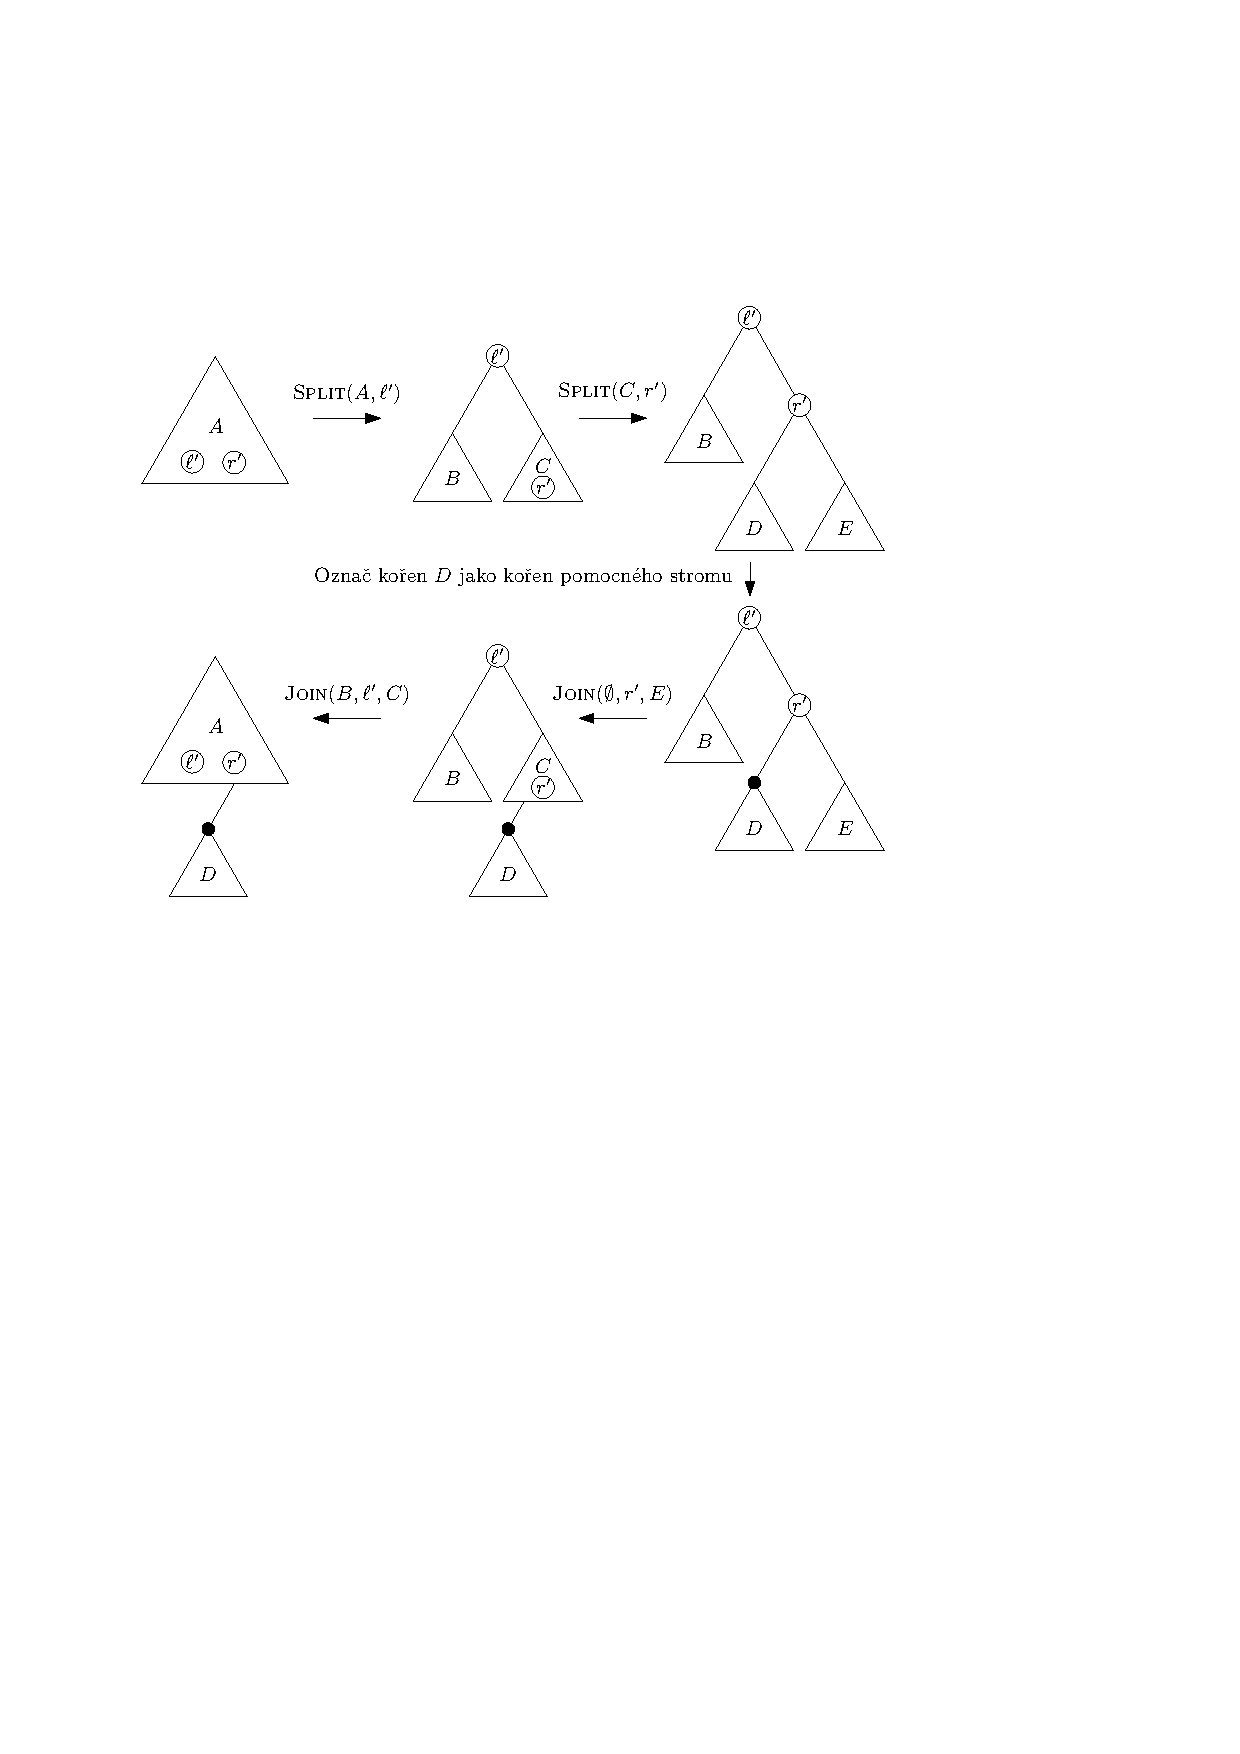
\includegraphics[width=.9\linewidth]{../img/cut_tango}
\caption{Rozdělení pomocných stromů} 

\label{obr:cut_tango} 
 
\end{figure}


Přitom vrcholy označené jako kořeny pomocných stromů považujeme za externí.
Dále najdeme předchůdce $\ell'$ vrcholu $\ell$ a následníka $r'$ vrcholu $r$. Poté zavoláme
$\ope{Split}(A, \ell')$ a dostaneme strom $B$ s~hodnotami menšími než $\ell'$,
samostatný vrchol $\ell'$ a strom $C$ s~hodnotami většími než $\ell'$. Poté
zavoláme $\ope{Split}(C,r')$ a dostaneme $D$, $r'$ a $E$. Nyní označíme kořen
$D$ za kořen pomocného stromu a připojíme ho jako levého syna vrcholu $r'$.
Dále zavoláme $\ope{Join}(\emptyset, r' E)$ a dostaneme opět strom $C$, ač
uspořádaný jinak než původně. Nakonec zavoláme $\ope{Join}(B,\ell',C)$ a
dostaneme strom $A$ s~provedenými požadovanými úpravami. V~celé operaci jsme
dvakrát hledali, dvakrát provedli \ope{Join}, dvakrát \ope{Split} a jednou
použili každou z~operací \ope{Pred} a \ope{Succ}, provedli jsme tedy $\o(1)$ operací, z~nichž každá trvá
$\o(\log |A|)\subseteq \o(\log\log n)$, celé rozdělení tedy trvalo
$\o(\log\log(n))$.


\section{Multisplay stromy}

\citet{multisplay} představili multisplay strom -- datovou strukturu, která se
snaží spojit dobré vlastnosti splay stromů a tango stromů. Tato struktura je
stále $(\log\log n$)-kompetitivní, ale na rozdíl od tango stromu dosahuje
amortizovaně $\o(\log n)$ na přístup (s~worst-case $\Theta(\log^2 n)$ na
přístup). Také dokáže vykonat průchod všemi prvky v~jejich pořadí v~čase
$\Theta(n)$ (na což tango strom potřebuje $\Theta(n\log\log n)$). Na rozdíl
od tango stromu bude navíc podporovat operace \ope{Insert} a \ope{Delete}\footnote{Úpravu modelu,
kterou potřebujeme k~tomu, abychom mohli mluvit o~optimalitě a kompetitivitě
struktury, která podporuje tyto operace, popíšeme později.}.

Myšlenka multisplay stromu je podobná, jako myšlenka tango stromu, pouze jako
pomocné stromy nepoužívá červenočerné stromy, ale splay stromy. Vzhledem
k~tomu, že jediné operace červenočerných stromů, které tango strom využívá, jsou
\ope{Split} a \ope{Join}, lze v~tango stromech nahradit červenočerné stromy
splay stromy přímočaře, protože splay stromy tyto operace také implementují.
Samotný postup vyhledání se od tango stromu nepatrně liší. Při vyhledávání
hodnoty v~multisplay stromu nejprve najdeme odpovídající vrchol $v$ bez
jakýchkoli úprav struktury stromu a až při cestě zpět do kořene postupně
zdola nahoru měníme preferované směry vrcholů. Po změně všech preferovaných
směrů nakonec ještě změníme preferovaný směr vrcholu $v$.

Samotné měnění preferovaných směrů je v~multisplay stromu o~poznání jednodušší než v~tango stromu.
Mějme vrchol $v$ ve stromu $T$, kterému chceme změnit preferovaný směr bez újmy
na obecnost zleva doprava. Potom nám stačí nejprve zavolat \ope{Splay$(v)$}.
Následně v~levém podstromu $v$ najdeme pomocí informace o~minimální hloubce
v~podstromu daného vrcholu vrchol $\ell$, který je vrcholem s~nejvyšší hodnotou
v~tomto stromu s~hloubkou menší než $v$. Pak zavoláme \ope{Splay$(\ell)$} na levý
podstrom $v$ (tak, aby $v$ zůstal kořenem pomocného podstromu a $\ell$ se
stal jeho levým synem). Dále v~rámci pravého podstromu $v$ zavoláme \ope{Splay}
na následníka $v$. Tím se část stromu, kterou chceme z~pomocného stromu
odstranit, stala pravým podstromem levého syna kořene a pomocný strom, který
chceme nově připojit, se stal levým podstromem pravého syna kořene. Stačí tedy
upravit příznak kořene pomocného stromu v~kořenech těchto podstromů a máme
hotovo. Rozmyslíme si, že dokonce ani není potřeba upravovat hodnoty minimální
hloubky vrcholu v~podstromu kořene či jeho synů (kvůli změně příznaků; samy
předchozí operace \ope{Splay} mohou vést k~nutnosti úpravy pomocných dat).
Maximální hloubky by sice mohlo být potřeba upravit, ale ty pro algoritmus
multisplay stromu nepotřebujeme -- nebudeme je tedy ve vrcholech
udržovat.

Nyní představíme úpravy struktury, které je potřeba provést, aby bylo možné do
struktury vkládat prvky.  Pokud do multisplay stromu $T$ vložíme prvek $p$, je
nutné ho vložit i do stromu $P$. Pokud v~binárním vyhledávacím stromu vyhledáme
prvek, který v~něm není, projdeme po cestě obsahující oba jeho sousedy, přičemž
jednomu z~nich bude chybět na příslušné straně syn. To znamená, že do
multisplay stromu můžeme vložit prvek tak, že použijeme standardní algoritmus
pro vkládání do binárního vyhledávacího stromu. Vkládaný prvek nejprve označíme
za kořen (jeho vlastního jednoprvkového) pomocného stromu. Při vkládání jsme prošli
jak jeho předchůdce, tak následníka. Na hlubším z~nich musí ale vrchol $v$
s~hodnotou $p$ viset i ve stromu $P$. Vrchol $v$ má tedy v~$P$ hloubku o~jedna vyšší,
než hlubší z~těchto dvou vrcholů. Minimální hloubky v~podstromech se tím
žádnému vrcholu (krom $v$) nezměnily, není je tedy potřeba opravovat. Nakonec
ve stromu přepneme preferované syny stejně jako při operaci \ope{Find}.

Tento postup má však jednu vadu -- všechny výše uvedené závisí na tom, že
$P$ má hloubku $\Theta(\log n)$. Protože o~$P$ jsme dosud mluvili jako
o~nevyvažovaném stromu, mohli bychom tuto vlastnost operací \ope{Insert} rozbít.
Proto je potřeba, aby $P$ byl vyvažovaný strom. Konkrétně zvolíme červenočerný
strom, protože pro nás bude výhodné, že má amortizovaně $\o(1)$ změn barev a
worst-case $\o(1)$ rotací na operaci. V~každém vrcholu si budeme nově pamatovat
jeho barvu v~$P$ a hodnoty\footnote{Bylo by lepší, kdybychom si mohli pamatovat
přímo ukazatele na příslušné vrcholy v~$T$ (byť amortizovaná i worst-case složitost zůstane zachována). Tím bychom ale
porušili pravidla modelu, která povolují v~každém vrcholu pouze dva ukazatele,
a to na syny daného vrcholu.} jeho rodiče a synů v~$P$. 

Nyní potřebujeme umět v~$T$ provádět úpravy nutné při vyvažování $P$. To
znamená, že musíme být schopni v~$T$ najít potomka a rodiče vrcholu v~$P$ a provádět
rotaci hran. Hledání rodiče a potomka vrcholu je snadné -- rozmyslíme si, že
cesta mezi libovolným vrcholem a jeho libovolným potomkem vždy navštíví nejvýše
dva různé pomocné stromy. Protože známe hodnotu uloženou v~hledaném rodiči či
potomkovi, najdeme ho vždy pomocí nejvýše dvou operací \ope{Find} v~pomocných
stromech. Jedno nalezení potomka či následníka tedy trvá amortizovaně
$\o(\log\log n)$ (včetně změny preferovaného vrcholu, pokud příslušná cesta
vedla napříč dvěma pomocnými stromy).

Při rotaci nás čeká několik problémů. Prvním z~nich je, že musíme zachovat
invariant, že každý vrchol má právě jeden preferovaný směr. To vyřešíme změnou
preferovaných směrů. Pokud chceme například provést rotaci hrany ve vrcholu
$v$, který je v~$P$ pravým synem vrcholu $w$, musíme nastavit preferovaný směr
vrcholu $v$ doleva a preferovaný směr vrcholu $w$ doprava. Tak dosáhneme toho,
že se při rotaci nezmění, které vrcholy náleží které preferované cestě,
může se změnit pouze jejich pořadí na ní.

Další změny struktury $P$ už se projeví pouze změnami pomocných informací
v~$T$, nikoli však změnou struktury. Tím nemáme na mysli, že bychom neprováděli
žádné rotace hran -- ještě nás čeká několik dílčích vyhledání, během nichž
provádíme v~pomocných stromech standardně operace \ope{Splay}. Již se nezmění
rozložení vrcholů mezi pomocnými stromy.

Samu rotaci pak provedeme úpravou hodnot rodičů a dětí v~dotčených vrcholech
(konkrétně je potřeba opravit vrchol, v~němž provádíme rotaci, jeho rodiče,
prarodiče a jednoho z~potomků). Dále opravíme hloubku vrcholů koncích rotované hrany. Problém ale spočívá v~tom, že nyní bychom
potřebovali opravit hloubku ve velké části stromu (například v~příkladu výše
zvýšit hloubku v~celém podstromu levého syna $\ell$ vrcholu $w$ a snížit
v~podstromu pravého syna $p$ vrcholu $v$). Všimneme si ale, že vzhledem
k~nastavení preferovaných směrů ve vrcholech $v$ a $w$ tvoří podstrom vrcholu
$\ell$ v~$P$ tytéž vrcholy jako podstrom kořene $r$ pomocného stromu
obsahujícího $\ell$ v~$T$. Podobně podstrom vrcholu $p$ v~$P$ je podstromem
kořene některého pomocného stromu v~$T$. Tyto kořeny najdeme tak, že budeme
z~kořene pomocného stromu obsahujícího $v$ a $w$ postupně hledat hodnoty
vrcholů $p$ a $\ell$, ale vždy vrátíme první vrchol s~příznakem kořene, který
najdeme (krom vrcholu, z~nějž hledat začínáme).

Nyní nahlédneme, že již dokážeme změny hloubek vyřešit v~konstantním čase pomocí některé
z~běžných technik, jako je například líná propagace změn směrem dolů, nebo, jak si
vybrali autoři multisplay stromu, diferenční kódování hloubky. To znamená, že
pouze kořen celého multisplay stromu zná svou hloubku. Ostatní vrcholy znají
rozdíl své hloubky v~$P$ a hloubky v~$P$ svého rodiče v~$T$. Stejným trikem
vyřešíme přepočítání informace o~minimální hloubce v~podstromu -- všimneme si, že
v~pomocném stromu obsahujícím $v$ a $w$ změnily hloubku pouze tyto dva vrcholy.
Proto stačí informaci přepočítat v~týchž vrcholech, jako v~případě hloubky, a
dále na cestě mezi $v$ a $w$.

Protože jsme popsali obecně, jak vykonat změnu barvy vrcholu a rotaci hrany ve
stromu, máme vše i pro implementaci operace \ope{Delete} v multisplay
stromech\footnote{Pokud se chceme co nejpřesněji držet modelu, který jsme
zavedli, přesouvání hodnot při mazání vnitřních vrcholů tak, jak je v~binárním
vyhledávacím stromu obvyklé, není možné. Proto musíme \ope{Delete} vrcholu,
který má nějaké potomky, implementovat tak, že nejprve provedeme rotace tak,
aby se tento vrchol stal listem, až potom ho smažeme.}. Nyní bychom rádi ukázali,
že i tyto úpravy jsou staticky optimální. To je ale problematické -- náš model
nepočítal s~vkládáním a mazáním. Proto ho musíme nadefinovat znovu.

Nyní již tedy přístupová posloupnost $S$ není pouze posloupností prvků
univerza, ale posloupností operací $\ope{Find}(x)$, $\ope{Delete}(x)$ a
$\ope{Insert}(x)$, kde $x$ musí náležet univerzu. Modelu nově dovolíme dvě
nové operace, a to vložení listu na místo chybějícího syna aktuálního vrcholu,
a odstranění listu (a označení jeho rodiče za aktuální vrchol). Po každém
stromu budeme vyžadovat, aby se při vykonávání operace \ope{Find} dotkl daného
vrcholu. Dále aby při operaci \ope{Insert} navštívil (v~tomto pořadí, byť na
asymptotické chování tento požadavek nebude mít vliv) vrcholy obsahující
předchůdce a následníka vkládaného prvku a nakonec skutečně vytvořil list
s~příslušnou hodnotou. Tento požadavek je adekvátní, protože každý binární
vyhledávací strom musí oběma těmito prvky projít při vkládání. Nakonec budeme
požadovat, aby strom při operaci \ope{Delete} navštívil předchůdce mazaného
vrcholu, mazaný vrchol a nakonec následníka mazaného vrcholu. Vzhledem k~tomu,
že mazat umíme pouze listy, musíme vždy odstraňovaný vrchol rotacemi přesunout
do listu, což opět znamená, že stejně musíme předchůdce i následníka navštívit.
Tento model je již dobře nadefinovaný, proto v~něm dává smysl nadefinovat optimální strom stejně, jako v~modelu předchozím.
Pro tento model \citet{multisplay} dokázali následující větu:

\begin{veta}[Dynamic Interelave Bound]
\def\dib{\operatorname{DIB}}
Mějme referenční strom $P$. V~tomto stromu má každý vrchol svůj preferovaný
směr, buď doprava nebo doleva. Vždy, když z~vrcholu při vyhledání prvku vyrazíme
jiným než preferovaným směrem, změníme preferovaný směr tohoto vrcholu. Strom
$P$ také podporuje rotace hran a operace \ope{Delete} a \ope{Insert} (které
probíhají standardním algoritmem binárního vyhledávacího stromu\footnote{Platí,
že standardní algoritmus na mazání nezapadá do nadefinovaného modelu. To
znamená, že celý náš referenční strom nebude zapadat do modelu dynamického
binárního vyhledávacího stromu. To nevadí, strom $P$ je pomyslný a strom
$T$, který skutečně stavíme, jeho chování pouze simuluje.}). Nechť $\dib(S)_P$ je
počet změn preferovaných směrů všech vrcholů v~$P$ při vykonávání posloupnosti
operací $S$, přičemž mezi některými operacemi mohly proběhnout rotace některých
hran. Potom $$\opt(S) \in \Omega(\dib_P(S)/2 - n - 2k + cm),$$ kde $P$ je
pomocný strom včetně popisu rotací, které provádíme mezi přístupy, a dalších
změn vzniklých vkládáním a mazáním, $n$ je počet vrcholů $P$ po poslední operaci, $k$
je počet rotací hran v~popisu $P$, $c$ je vhodně zvolená kladná konstanta a $m$
je délka posloupnosti $S$.  \end{veta}

Nahlédneme, že vzhledem k~výše uvedenému popisu mazání a vkládání je multisplay strom i v~dynamickém modelu stále $\log\log(n)$-kompetitivní. 

%\section{Geometrický náhled na stromové operace}

%%% Fiktivní kapitola s ukázkami citací

\chapter{Cíle práce}

Cílem práce je určit, která struktura binárního vyhledávacího stromu je v~praxi nejefektivnější, kde efektivitu budeme měřit jednak počtem navštívených vrcholů, jednak časem běhu při vykonávání několika konkrétních posloupností. Zkoumat budeme červenočerný strom, splay strom, tango strom a multisplay strom. Budeme postupovat následovně:

\begin{enumerate}
\item Vytvoříme implementaci řečených datových struktur v~jazyce C.
\item Navrhneme několik sad syntetických přístupových posloupností pro různě velké datové struktury.
\item Změříme chování implementací datových struktur na sadách posloupností. Poté provedeme diskusi.
\item Nalezneme program, který obsahuje implementaci nějakého binárního vyhledávacího stromu. S~pomocí tohoto programu vyrobíme přístupovou posloupnost z~reálného světa. S~touto posloupností budeme opakovat předchozí bod.
\end{enumerate}

\chapter{Metodika}

V~této kapitole popíšeme některé detaily implementací binárních vyhledávacích stromů, které vznikly pro potřeby této práce (ne však jejich rozhraní -- to popíšeme později v~příloze práce). Dále popíšeme metodiku měření času a počtu dotčených vrcholů.

\section{Implementace}

Všechny testované struktury jsme implementovali v~jazyce C. Ten byl zvolen
proto, že umožňuje kontrolovat, co přesně měříme. Měření nám nepokazí ani
interní fungování interpreteru, což by hrozilo, kdybychom zvolili například
Python, ani zásahy garbage collectoru, kterým bychom se nevyhnuli například
v~Javě.

Při implementaci testovaných struktur jsme pro každou strukturu
naimplementovali operaci \ope{Find}. Dále jsme pro červenočerný strom a splay
strom napsali operaci \ope{Insert}, pro zbylé dva stromy potom operaci
\ope{Build}. Protože ale stavbu struktury nechceme měřit,  vybudujeme před měřením
červenočerný a splay strom struktury nejprve tím, že do z počátku prázdné struktury
postupně vložíme všechny klíče, které mají obsahovat, v~rostoucím pořadí. Tento postup jsme obzvláště u~červenočerného stromu zvolili záměrně, abychom dostali na začátku pokud možno co nejhůře vyvážený červenočerný strom.

Od reálného použití (přinejmenším červenočerného a splay stromu) jsme se mírně
odchýlili metodou alokace paměti na nové vrcholy -- abychom dosáhli co
nejpředvídatelnějšího chování, alokujeme jedno pole vrcholů se začátkem
zarovnaným na stránku paměti a vrcholy budeme mít uložené v~něm. Adresy nových
vrcholů v~rámci tohoto pole jsme nejprve přiřazovali sekvenčně, ale po
zjištěních ze sekce \ref{sec:rb_and_cache} jsme, počínaje měřeními popsanými
v~sekci \ref{sec:sequential_access_sequence}, přiřazovali pro červenočerný strom
adresy v~náhodném pořadí. 

Dále jsme se odchýlili od modelu -- ve snaze minimalizovat množství paměti
zabírané jednotlivými vrcholy jsme se rozhodli neukládat ve vrcholech ukazatele na
rodiče a místo toho si ukazatele na rodiče všech vrcholů mezi aktuálním
vrcholem a kořenem držet na zásobníku. Čistě pro zjednodušení algoritmu jsme se
také rozhodli operace \ope{Split} a \ope{Join} červenočerného stromu, které
jsou interně využívány operací \ope{Find} tango stromu, neimplementovat pomocí
rotací hran, ale přímo tak, jak byly popsány v~sekci o~červenočerném stromu. 

\citet{tango} ve svém článku o~tango stromu mluví mimo jiné o~tom, že jako
součást přístupu vždy změní preferovaný směr v~cílovém vrcholu na směr doleva.
Protože však tato změna není pro důkazy složitosti tango stromu nutná, rozhodli
jsme se ji neprovádět (naopak změna preferovaného směru v~cílovém vrcholu
multisplay stromu nutná je, tu tedy provádíme).

Všechny ostatní implementační problémy řešíme přímočaře přesně podle popisu
v~první kapitole této práce a v příslušných článcích.

\section{Měření}

Měření počtu dotčených vrcholů jsme provedli tak, že jsme každé operaci \ope{Find}
přiřadili její pořadové číslo. V~každém vrcholu jsme si zaznamenali pořadové číslo
operace, při které byl naposled navštíven. Poté jsme vždy, když jsme se dotkli daného
vrcholu (dotekem vrcholu myslíme dereferencování na něj mířícího ukazatele),
zkontrolovali, zda jsme ho během této operace již viděli. Pokud ne, změnili jsme
číslo poslední operace, které máme v~tomto vrcholu zaznamenané, a zvýšili
počítadlo dotčených vrcholů o~jedna.

Měření času jsme provedli pomocí jiného programu, než kterým počítáme doteky
(experimentálně jsme totiž zjistili, že samo počítání doteků násobně zpomaluje
běh). Stejně jako v~případě počtu doteků používáme naši implementaci datových
struktur, jejíž zdrojový kód je součástí elektronických příloh práce. K~její
kompilaci jsme použili překladač {\tt gcc} ve verzi {\tt 10.2.1} s~úrovní
optimalizací {\tt O3}. Při měření času jsme postupovali tak, že jsme rourou propojili standardní výstup generátoru (jehož zdrojový kód je
taktéž součástí elektronických příloh práce) a standardní vstup testovaného
programu. V~testovacím programu poté nejprve vybudujeme
strukturu patřičné velikosti, potom načteme ze standardního vstupu do pole
prvních nejvýše $10^7$ prvků přístupové posloupnosti. Pak začneme měřit
čas a vykonáme načtenou část přístupové posloupnosti. Pokud ještě zbývá
nenačtená část posloupnosti, měření přerušíme, načteme dalších nejvýše
$10^7$ prvků a změříme tuto část posloupnosti. Takto pokračujeme, dokud
se nedostaneme na konec posloupnosti.

Procesorový čas jsme měřili pomocí funkce {\tt clock()} z~hlavičkového souboru
{\tt time.h}. K~měření jsme použili procesor {\tt AMD EPYC 7301}
s~frekvencí  $2.7\, \operatorname{GHz}$. Tento procesor obsahuje 16 fyzických a tedy
32 logických jader, naše měření však nebylo nijak paralelizováno. Jedno jádro má k dispozici $64\,\operatorname{kB}$ L1 cache, $512\,\operatorname{kB}$ L2 cache a $8\,\operatorname{MB}$ L3 cache. Procesory však mohou využívat i L3 cache patřící jiným procesorům; součet kapacit všech L3 cachí v systému je $128\,\operatorname{MB}$. V~systému bylo
k~dispozici $126\,\operatorname{GB}$ RAM. Vzhledem k~tomu, že na pamětově
nejnáročnější z~navržených testů stačilo méně než $10\,\operatorname{GB}$
paměti, nás tedy dostupná paměť nijak neomezila. Měření proběhlo pod operačním
systémem {\tt Debian GNU/Linux 11}.

Měření času jsme systematicky neopakovali, ale na základě několika pokusů jsme dospěli k závěru, že rozptyl mezi více měřeními téže přístupové posloupnosti je zanedbatelný.

%\chapter{Výsledky}

V této kapitole popíšeme chování naší implementace stromů na několika třídách přístupových posloupností.

\section{Náhodná přístupová posloupnost}

Třída náhodných přístupových posloupností vypadá tak, že pro danou velikost
strom vyrobíme náhodnou posloupnost přirozených čísel z intervalu $[0,n)$.
Náhodná čísla generujeme pomocí pseudonáhodného generátoru {\tt xoshiro256++},
který představili \citet{xoshiro}. Pro měření jsme zvolili velikosti stromů od $10$ do $1\cdot
10^8$, kde každá další testovaná velikost byla $\sqrt[7]{10}$-krát větší, než ta předchozí. Takovýto krok
jsme zvolili proto, že s ním v celém rozsahu měříme celkem 50 různých velikostí
stromu, tedy dosáhneme rozumného kompromisu mez počtem vzorků a celkovou
dobou měření. 

Délka posloupnosti byla vždy $\max(1\cdot10^7, 10\cdot n)$.
Takové číslo jsme zvolili proto, abychom snížili pravděpodobnost, že dostaneme
náhodnou posloupnost, jejíž čas běhu a počet dotyků na operaci budou daleko od
příslušné střední hodnoty, abychom i pro větší $n$ alespoň jednou navštívili
téměř všechny prvky a aby
nepřesnost měření času (která může dosahovat až řádově desítek milisekund)
nehrála významnou roli v celkovém času vykonávání posloupnosti. 

\def\graphfigure#1#2{
\begin{figure}[h!]
\centering
 \makebox[\textwidth][c]{\includegraphics{graphs/#1}}
\caption{#2}
\label{obr:#1}
\end{figure}
}

\graphfigure{touch_r}{Doteky vrcholů -- náhodná přístupová posloupnost.}


Při vlastním měření jsme ale neměřili dvě nejvyšší hodnoty $n$ pro tango strom kvůli vysoké časové náročnosti měření.

Na základě teorie bychom čekali, že počet doteků na operaci u multisplay, splay a červenočerného stromu poroste logaritmicky s počtem vrcholů, u tango stromu ještě s faktorem $\log\log$ navíc, což měření potvrzují, viz obrázek \ref{obr:touch_r}.
\let\oldlog\log
\def\log{\oldlog_2}

Na grafu vidíme, že červenočerný strom potřebuje konzistentně přibližně $(\log
n) - 1/2$. $\log n$ jsme do grafu přidali pro porovnání. To zní podezřele --
pro červenočerný strom je střední hodnota počtu doteků na operaci z náhodné
přístupové posloupnosti prostě průměrná hloubka vrcholu (kde kořen má hloubku
1). Dokonale vyvážený strom na $n$ vrcholech má průměrnou hloubku vrcholu
vrcholu $(\log n) - 1 + o(1)$. My jsme ale v minulé kapitole řekli, že náš
červenočerný strom je tak nevyvážený, jak je jen možné.

Jak je tedy možné, že průměrná hloubka vrcholu ve velmi nevyváženém
červenočerném stromu je jen o aditivní $1/2$ větší než v dokonale vyváženém
stromu? Odpověď na tuto otázku je v nejasné definici velmi nevyváženého stromu.
Náš strom vypadá tak, že na jeho pravé páteři se střídají černé a červené
vrcholy, ale celý zbytek stromu krom této cesty a vrcholů s ní bezprostředně
sousedících je stále černý\footnote{Toto tvrzení dokážeme později.}. Proto je i vyvážený, jak to jen jde -- kvůli
invariantu červenočerného stromu je každý čistě černý podstrom dokonale
vyvážený.

Náš strom je
tedy extrémně nevyvážený v tom smyslu, že dosahuje co nejvyšší možné maximální
hloubky při daném počtu vrcholů. Také je extrémně nevyvážený stran poměru
velikosti pravého a levého podstromu kořene (v závislosti na přesné velikosti
experimentálně určeného jako $2:3$ až $1:4$). Protože však současně jsou
podstromy všech vrcholů krom těch ležících na pravé páteři dokonale
vyvážené, stran průměrné hloubky vrcholu je takto vybudovaný strom poměrně
blízko dokonale vyváženému stromu.


Splay strom potom potřebuje zhruba $1.28\cdot \log n$ doteku na přístup, multisplay strom
dokonce $3.35\cdot \log n$. U tango stromu jsme na našem vzorku naměřili v
průměru $4.88\cdot \log n$ doteků, což ale není příliš zajímavé -- u ostatních
stromů očekáváme, že bude počet doteků na operaci dělený logaritmem velikosti stromu konvergovat
k nějaké konstantě, u tango stromu toto očekávání nemáme. Nejvyšší zaznamenaný
počet dotyků pro tango strom byl v testu pro $n \cong 5.18\cdot 10^7$. V tomto
testu jsme naměřili asi $6.81\cdot \log n$ doteků na operaci. Pro srovnání,
$\log\log 5.18\cdot 10^7 \cong 4.68$. 

Dále si všimneme mírného rozvlnění křivky tango stromu kolem $n=5\cdot 10^3$ a
znovu kolem $n=1\cdot 10^6$. Tento efekt se ale výrazněji projeví při
sekvenčních přstupech, které budeme diskutovat v následující sekci, s jeho
vysvětlením tedy počkáme tam.

\graphfigure{time_r}{Průměrný čas na operaci -- náhodná přístupová posloupnost.}

Na obrázku \ref{obr:time_r} vidíme naměřené časy. Proti obrázku \ref{obr:touch_r}
se křivka tango stromu ještě trochu vzdálila ostatním. Dále vidíme zlom všech
křivek pro $n$ mezi $1\cdot10^6$ a $1\cdot 10^7$. Vzhledem k tomu, že použitý
procesor má $128\,\operatorname{MB}$ L3 cache a jeden vrchol  červenočerného či
splay stromu zabírá v paměti 24 bytů, přibližně při $3\cdot 10^6$ vrcholech se již
strom nevejde do cache současně s $40\,\operatorname{MB}$, které zabírá načtená
část přístupové posloupnosti. Přibližně při $5\cdot10^6$ vrcholech se pak již strom nevejde do cache ani sám.
Jeden vrchol multisplay stromu a tango stromu pak zabírá 32 bytů a výše uvedené pro ně platí obdobně. 

\graphfigure{ratio_r}{Průměrný čas na dotyk -- náhodná přístupová posloupnost.}

\subsection{Červenočerný strom a cache}

Překvapivé je, že kolem $n=2\cdot10^6$ se splay strom stává rychlejší než
červenočerný strom. Ve skutečnosti se podle grafu na obrázku \ref{obr:ratio_r}
průměrný čas na dotek vrcholu v červenočerném stromu propadá až téměř na úroveň tango
stromu -- to je obzvláště překvapivé proto, že červenočerný strom vrcholy pouze
prochází a nijak strom nemodifikuje, kdežto všechny ostatní stromy vrcholy
modifikují a navíc jimi mohou projít během jedné operace i vícekrát, což my
ovšem ale stále počítáme jako jeden dotyk.

Toto chování má své vysvětlení, předtím, než k němu přistoupíme ale musíme
udělat krátkou odbočku, v níž vysvětlíme, jak funguje cache procesoru.

\subsubsection{Chování cache}

Procesor má obvykle tři úrovně cache, nejmenší L1, o něco větší L2 a největší
L3. To pro nás ale teď nebude důležité -- omezíme se pouze na jednu úroveň.
Cache je rozdělená na jednotlivé řádky, v dnešních procesorech typicky 64 bytů
velké. Pokud procesor chce přistoupit na nějakou adresu, blok paměti o
velikosti jednoho cachového řádku zarovnaný na velikost cachového
řádku\footnote{To znamená, že adresa začátku tohoto bloku je dělitelná délkou
cachového řádku.} obsahující tuto adresu je načten do cache. Může se ale stát,
že v cachi už není volné místo. V ideálním světě by v takovém případě cache
vybrala z řádků, které obsahuje, ten, ke kterému procesor nejdéle nepřistoupil,
a ten by odstranila. Tomuto přístupu obecně říkáme \emph{LRU\footnote{Z
anglického \emph{least recently used}.} cache}.

Pro to bychom ale potřebovali, aby libovolný řádek cache mohl obsahovat
libovolný blok paměti. Takovou cache bychom nazvali \emph{plně asociativní}.
Potom by ale bylo velmi obtížné zjistit, kde v cachi je daný blok paměti
uložený. Proto jsou v praxi cache \emph{$k$-cestně asociativní}. To znamená, že
každý blok může být uložen pouze na $k$ různých místech v cachi. Která místa to
budou je pak určeno několika nejnižšími bity adresy bloku. Konkrétně pokud máme
cache o $C$ bytech, uložení bloku určuje $\log (C/k)$ nejnižších bitů jeho
adresy.

To znamená, že pokud jsou dva bloky paměti uložené na adresách, které dávají
stejný zbytek po dělení dostatečně velkou mocninou dvojky, mají oba na výběr
pouze $k$ míst v cachi, kam mohou být uloženy. Navíc se jedná o těch samých $k$
míst. Tomu říkáme, že tyto bloky, případně adresy, \emph{aliasují}.

Kdybychom potřebovali pracovat s větším počtem aliasujících bloků, přestává být
podstatný celkový počet řádků, které se do cache vejdou -- o tom, jak úspěšná
cache bude, rozhoduje pouze hdnota $k$.

\subsubsection{Cache a dokonale vyvážené stromy}\label{sec:cache_and_balanced}

Nyní se vrátíme k červenočerným stromům. Již dříve jsme řekli, že náš postup stavby červenočerného stromu vede k tomu, že podstrom každého vrcholu krom vrcholů na pravé páteři je dokonale vyvážený. Proto můžeme pro zjednodušení problém vysvětlit na dokonale vyváženém stromu. Pro strom, který dostaneme z naší konstrukce červenočerného stromu budou závěry, které uděláme, platit podobně. Jediná důležitá věc, které si ještě musíme všimnout, je, že náš způsob alokace paměti spolu s naším způsobem stavby stromu vede k tomu, že vrcholy jsou v paměti uloženy jeden za druhým v rostoucím pořadí.

Mějme tedy dokonale vyvážený strom nad množinou klíčů $[2^k-1]$. Všimneme si že v listech jsou uložena právě lichá čísla. V jejich rodičích jsou uložena právě čísla, která dávají zbytek 2 po dělení 4. V jejich rodičích pak čísla, která dávají zbytek 4 po dělení 8. Takto bychom mohli pokračovat dál až k tomu, že v kořeni je právě číslo, které dává zbytek $2^{k-1}$ při dělení $2^k$ (mimo jiné proto, že v kořeni je přesně číslo $2^{k-1}$).

Na to se můžeme ale podívat i opačně, shora dolů. Nahlédneme, že v kořeni je právě číslo dělitelné $2^{k-1}$. V kořeni a jeho synech jsou pak dohromady právě všechna čísla dělitelná $2^{k-2}$. Podobně můžeme pokračovat dál -- všimneme si, že v prvních $h$ hladinách jsou uložena právě všechna čísle, která jsou dělitelná $2^{k-h}$. A jsou-li tedy vrcholy uložené za sebou v rostoucím pořadí jejich klíčů, a navíc předpokládáme, že množství bytů v paměti, které jeden vrchol zabírá, je dělitelné 8 (tento předpoklad splňují všechny naše implementace stromů), potom adresy všech vrcholů z prvních $h$ hladin dávají po dělení $2^{k-h+3}$ stejný zbytek.

Nyní se zamyslíme, jaké chování cache bychom si přáli při vykonávání náhodné přístupové posloupnosti nad dokonale vyváženým binárním vyhledávacím stromem. Pravděpodobnost návštěvy vrcholu $v$ při daném přístupu je přesně rovna velikosti jeho podstromu dělené počtem vrcholu ve stromu. To znamená, že tato pravděpodobnost je klesající funkce hloubky tohoto vrcholu. My bychom si přáli držet si v cachi (samozřejmě za podmínky, že máme příliš malou cache, než aby se nám do ní vešel celý strom) právě vrcholy, které mají pravděpodobnost přístupu alespoň $p$ pro vhodně zvolené $p$. Rozmyslíme si, že (opět pro dostatečně velký strom) není možné, že bychom do jednoho řádku cache uložili více zajímavých vrcholů (například v našem případě -- vrcholy stromu jsou 24 bytové, řádky cache 64 bytové. I kdybychom do jednoho řádku uložili 3 vrcholy, oba sousedi libovolného vrcholu $v$ s nízkou hloubkou jsou listy, a jejich sousedé různí od $v$ jsou jejich rodiče). Proto prostě chceme do cache uložit prvních $h$ hladin stromu pro vhodně zvolené $h$.

Jak jsme ale již ukázali, pokud má strom celkem $\ell$ hladin, prvních $h$
hladin obsahuje vrcholy, jejichž adresy jsou kongruentní modulo $2^{\ell - h}$.
Pokud naše cache má kapacitu $2^c$ bytů a je $k$-asociativní, budou tyto adresy
rozděleny pouze do $\max\left(1, 2^{c+h-\ell - 3}/k\right)$ tříd
ekvivalence aliasování, a současně jich tedy bude moct být uloženo nejvýše
$\max\left(k, 2^{c+h-\ell - 3}\right).$

Pokud do tohoto vzorce dosadíme náš hardware a náš největší měřený případ,
dostaneme dostaneme následující informace: Naše L3 cache má $128
\,\operatorname{MB}$. Jeden cachový řádek má 64 bytů. Naše cache má tedy
$2^{27}$ bytů a $2^{21}$ řádků. Proto bychom do ní rádi uložili prvních 21 hladin stromu. Náš
největší měřený případ měl $1\cdot 10^8 > 2 ^ {26}$ vrcholů. Z těchto ale
můžeme současně uložit jen $2^{27 + 21 - 26 - 3} = 2^{19}$, tedy jednu čtvrtinu
toho, co bychom mohli s plně asociativní cachí. Co hůře, všimneme si, že dokud
$2^h \geq 4k$, poměr mezi částí stromu, kterou bychom chtěli  uložit, a částí,
kterou se nám skutečně uložit povede, zůstává konstantní $1/4$. Jinými slovy,
nemůžeme doufat, že do cache tedy uložíme prostě o 2 hladiny méně, než jsme
doufali -- pokud bychom se pokusili uložit $2^{19}$ vrcholů z prvních 19
hladin, podaří se nám ve skutečnosti uložit pouze $2^17$ vrcholů. To znamená,
že z každé hladiny, která obsahuje více než $4k$ vrcholů, se nám podaří uložit
pouze čtvrtinu (stále se jedná o optimistický odhad, předpokládáme, že hladiny
mezi sebou třídy ekvivalence aliasování nesdílí, dostatečně blízko ke kořeni
však tento předpoklad nemusí platit). 

V našem případě se $k$ rovná $16$. To znamená, že můžeme plně uložit prvních pět hladin, z
šesté uložíme polovinu, ze všech dalších pak už jen čtvrtinu až po 23., což je
poslední hladina, z níž se jedna čtvrtina do cache vejde, i kdyby v ní nic
jiného než tato hladina nebylo. Na dalších úrovních pak zeshora odhadneme
pravděpodobnost přítomnosti daného vrcholu v cachi popořadě jako $1/8$, $1/16$
a tak dále. To znamená, že střední hodnota počtu nenacachovaných řádků, které
musíme načíst při přístupu k náhodnému listu stromu, je díky linearitě střední
hodnoty $$\sum_{h=1}^{26} \operatorname{P}[\text{Vrchol na $h$-té hladině není v
cachi}] > 5 \cdot 0 +  \frac 12 + 17\cdot \frac34 + \frac78 + \frac{15}{16} + \frac{31}{32} = 15\frac1{32},$$ což je výrazně horší než pět přístupů mimo cache, ve které bychom mohli doufat, kdyby naše cache byla plně asociativní.   

V tomto výpočtu jsme navíc
zanedbali další faktory, které nám mohou škodit -- do cache se musí vejít i
jiné věci, než prvních $h$ hladin stromu, jako třeba náš program, naše poslední
cesty stromem mimo prvních $h$ hladin, nebo aktuální kus přístupové
posloupnosti. Dále je potřeba si uvědomit, že podobný problém nastane na všech
úrovních cache.

\subsubsection{Praktické chování červenočerných stromů}

Tím bychom tedy měli vyřešené chování dokonale vyváženého stromu a můžeme se
vrátit k červenočernému stromu. Experimentálně jsme ověřili, že naší
implementací červenočerného stromu mají pro $n=1\cdot 10^7$  adresy vrcholů v
prvních 8 hladinách stromu, tedy 255 vrcholů nejblíže ke kořeni, všechny
stejných 17 nejnižších bitů. Více než polovina z nich se shodne dokonce na 19
bitech. Pro $n=1\cdot10^8$ mají adresy 255 nejvyšších vrcholů dokonce 21
společných nejnižších bitů.   

Dále jsem ověřili, zda problém skutečně nastává. Připomeneme, že naše struktury stavíme tak, že nejprve naalokujeme pole tak velké, aby se nám do něj vešel celý strom, jehož začátek je zarovnaný na začátek stránky paměti, a poté vždy, když potřebujeme nový vrchol, použijeme z tohoto pole první nepoužitý. Vzhledem k tomu, že jsme ani jedné ze struktur neimplementovali operaci \ope{Delete}, je tento postup poměrně přímočarý.

Díky naší implemntaci operací \ope{Build} u jednotlivých stromů vede tento postup k tomu, že splay strom a červenočerný strom mají své vrcholy v paměti v rostoucím pořadí klíčů, tango strom a multisplay strom v preorder pořadí jejich referenčních stromů $P$. To znamená, že je nejprve uložen kořen $P$, pak rekurzivně stejně jeho levý podstrom, a nakonec pravý podstrom.

Provedli jsme tedy experiment, kdy jsme opět naměřili čas běhu červenočerného stromu na náhodné přístupové posloupnosti. Upravili jsme ale alokaci paměti na nové vrcholy tak, že z pole nepřidělujeme adresy novým vrcholům sekvenčně, ale v náhodném pořadí. Tato úprava vedla k tomu, že průměrný čas na dotek mnohem lépe kopíruje chování splay stromu, jak je vidět na obrázku \ref{obr:randomized_rb}.

\graphfigure{randomized_rb}{Průměrný čas na přístup -- náhodná přístupová posloupnost.}

\subsubsection{Teoretické chování červenočerných stromů}

Nyní se ale ještě na chvíli vrátíme k výpočtům. Již víme, že popisovaný problém
skutečně v praxi nastává. V sekci \ref{sec:cache_and_balanced} jsme ukázali, že
perfektně vyváženého stromu, jehož počet vrcholů je mocnina dvojky mínus jedna,
se týká velmi výrazně. To má jednoduchý důvod -- takový strom je velmi
pravidelný, a tyto pravidelnosti jsou založené na mocninách dvojky, které také
figurují v ekvivalenčních třídách aliasování cache. Tango stromu, multisplay
stromu a splay stromu se tento problém vyhne právě kvůli tomu, že jejich
struktura je velmi nepravidelná (přestože u prvních dvou existuje dokonale
vyvážený refenční strom $P$. Možná jim v našem měření pomohly také
nepravidelnosti ve struktuře $P$ pramenící z toho, že žádná z měřených
velikostí nebyla příliš blízko k mocnině dvojky.)

Přirozená otázka pak ale je, nastávají tyto problémy stejnou měrou jako v
dokonale vyváženém stromě? Ukážeme, že rozdíly mezi červenočerným a dokonale
vyváženým stromem nám pomůžou zcela zanedbatelně -- téměř všechny vrcholy,
kterými budeme s velkou pravděpodobností potřebovat projít, budou stále na
adresách kongruentních modulo vysoká mocnina dvojky. 

Připomeneme, že
pravděpodobnost, že bude nutné projít daným vrcholem při vyhledání rovnoměrně náhodně vybraného klíče z tohoto stromu, je rovná velikosti
podstromu tohoto vrcholu dělené velikostí celého stromu. Dále vzhledem k tomu,
že uvažujeme sekvenční uložení vrcholů, nebudeme pracovat pro zjednodušení
práce s adresami vrcholů, ale s klíči v nich -- snadno nahlédneme, že klíče
dvou vrcholů jsou kongruentní modulo $2^h$, právě když jejich adresy jsou
kongruentní modulo $2^{h+s}$, kde $2^s$ je nejvyšší mocnina dvojky, kterou je
dělitelný počet bytů paměti, které zabírá jeden vrchol. Pak dokážeme
následující tvrzení:

\begin{tvrz}
Mějme červenočerný strom $T$, který vznikl tak, že byly jeho klíče vloženy do na počátku prázdného stromu v rostoucím pořadí. Potom pro každé $h\in \mathbb N$ jsou vrcholy, jejichž podstrom obsahuje alespoň $2^h -1$ vrcholů, až na konstantně mnoho výjimek právě ty vrcholy, jejichž klíče jsou kongruentní s klíčem v kořeni modulo $2^{h-1}$.
\end{tvrz}

\begin{dukaz}
Budeme předpokládat, že $T$ má alespoň $2^h-1$ vrcholů.

Nejprve začneme s důkazem, který jsme slíbili již na začátku této sekce.

\begin{lemma}
Mějme červenočerný strom $T$, který vznikl tak, že byly jeho klíče v rostoucím pořadí vloženy do na počátku prázdného stromu. Pak všechny červené vrcholy z $T$ leží buď na pravé páteři $T$, nebo jsou syni vrcholu, který leží na pravé páteři $T$.
\end{lemma}
\begin{dukaz}
Budeme postupovat indukcí podle počtu vrcholů $T$. Je zřejmé, že pro strom o jednom vrcholu tvrzení platí. Nyní ukážeme, že pokdu do takového stromu $T$ nad klíči $[n]$ vložíme klíč $n+1$, strom bude stále mít požadovanou vlastnost.

Rozmyslíme si, jak by se mohlo stát, že nám vznikne červený vrchol mimo pravou páteř nebo její sousedství. Není možné, že bychom ho tam tak přímo vložili, protože vkládáme nové maximum a tedy na pravou páteř. Při vyvažování po operaci \ope{Insert} děláme 3 typy kroků: Přebarvení černého vrcholu na červený a obou jeho synů z červené na černou, rotace a dvojitá rotace.

Při přebarvování se nám nemůže stát, že bychom přebarvili na červeno vrchol mimo pravou páteř, protože takto přebarvujeme vždy vrchol na cestě mezi vkládaným vrcholem a kořenem.

Při vkládání nového maxima se nám nikdy nemůže stát, že bychom potřebovali provést dvojitou rotaci, protože tu provádíme pouze v situaci, kdy při cestě z vkládaného vrcholu do kořene střídáme směry, ze kterých se vracíme.

Při vkládání nového maxima bychom mohli chtít provést jedině rotaci doleva.
Mějme tedy vrchol $v$, jeho pravého syna $u$ a levého syna $w$. Dále mějme levého syna $x$ vrcholu $u$.
rotovaná hrana vždy leží na cestě z nového vrcholu do kořene, víme, že $v$ a
$u$ leží na pravé páteři. Kdyby se nám po rotaci stalo, že budeme mít červený vrchol mimo pravou páteř $T$ a její sousedství, musel by před rotací být červený alespoň jeden z vrcholů $w$ a $x$. To ale není možné. Víme, že v případě, že jsme přistoupili k vyvažování, musí být vrchol $v$ černý a vrchol $u$ i jeho pravý syn červený. To znamená, že vrchol $u$ musel být červený již před aktuální operací \ope{Insert}. Kdyby tedy byl vrchol $x$ červený, porušoval by již před aktuální operací \ope{Insert} spolu s vrcholem $u$ invariant červenočerného stromu. Kdyby byl červený vrchol $w$, nevyvažovali bychom strom rotací, ale přebarvením $u$ a $w$ na černo a $v$ na červeno. 
\end{dukaz}

Z invariantu červenočerného stromu vyplývá, že pokud v červenočerném stromu nejsou krom možná kořene žádné červené vrcholy, musí být všechny cesty z kořene do externího vrcholu stejně dlouhé, tedy tento strom musí být dokonale vyvážený a počet vrcholů v něm musí být bez jednoho mocnina dvojky. To samé platí i o podstromech jednotlivých vrcholů v červenočerném stromu.

Před další částí důkazu nahlédneme, že v $T$ nikdy nemůže být pravý ani levý podstrom vrcholu menší, než pravý ani levý podstrom jeho syna, krom případu, kdy nějaké z těchto podstromů obsahují část pravé páteře $T$.

Mějme dva vrcholy $u$, $v$ stromu $T$ takové, že $u$ je bez újmy na obecnosti v pravém
podstromu $v$. Velikost levého podstromu $u$ si označíme jako $2^{h'}-1$. Rozmyslíme si, kde leží vrcholy, jejichž klíče leží mezi klíčem
$u$ a $v$. Jedná se jednak o celý levý podstrom $v$, jednak o některé vrcholy
na cestě mezi $u$ a $v$, a jednak o levé podstromy těchto vrcholů. Tyto vrcholy
sice potenciálně mohou ležet i na pravé páteři, ale kořeny všech zmíněných podstromů nikoli -- buď se jedná o levé podstromy, nebo se vše odehrává v levém podstromu $v$. To znamená, že velikost každého z těchto podstromů je alespoň $2^{h'} - 1$, a tedy pokud k ní připočteme ještě samotný vrchol, na kterém tento podstrom visí, bude dělitelná $2^{h'}$. To tedy znamená, že rozdíl mezi hodnotami v $u$ a $v$ je dělitelný $2^{h'}$.

\begin{pozorovani}\label{poz:1}
Tím jsme ukázali, že pro všechny vrcholy platí, že rozdíl jejich hodnoty a hodnoty kořene je dělitelný hodnotou jedna plus velikost pravého či levého podstromu daného vrcholu (v závislosti na tom, zda je daný vrchol v levém či pravém podstromu kořene).
\end{pozorovani}

Nyní najdeme vrchol $v$, což bude vrchol s nejvyšším klíčem takový, že jeho levý
podstrom má velikost alespoň $2^{h-1} -1$, nebo kořen, pokud žádný takový vrchol neexistuje. Rozmyslíme si, že $v$ leží na pravé páteři $T$. Strom si
rozdělíme na dvě části: $T_2$, což bude pravý podstrom $v$, a $T_1$ což bude zbytek $T$ včetně $v$.

Podmínky ze znění tvrzení si označíme jako $p_1$ a $p_2$. Vrchol tedy splňuje podmínku $p_1$, pokud jeho podstrom obsahuje alespoň $2^h-1$ vrcholů, a podmínku $p_2$, pokud je jeho hodnota kongruentní s hodnotou v kořeni modulo $2^{h-1}$.

Nyní ukážeme, že v $T_1$ splňují obě podmínky přesně tytéž vrcholy, a v $T_2$ splňuje každou z podmínek nejvýše konstantně mnoho vrcholů.

Pro $T_1$ tedy potřebujeme dokázat dvě implikace. První z nich, tedy že vrchol
splňující $p_1$ splňuje i $p_2$, plyne z pozorování \ref{poz:1}. Naopak pokud
máme vrchol $u$, který nesplňuje $p_1$, najdeme jeho nejbližšího předka $w$,
který $p_1$ splňuje. Rozmyslíme si, že $w$ nemůže ležet na pravé páteři. Tento vrchol má podstrom velikosti právě $2^{h}-1$. Rozdíl
jeho hodnoty a hodnoty libovolného vrcholu v jeho podstromě je tedy maximálně
$2^{h-1}-1$. Protože dále už víme, že $w$ splňuje i $p_2$, $u$ splňovat $p_2$
nemůže.

Na poslední část důkazu potřebujeme ještě jedno lemma.

\begin{lemma}
Každý vrchol $T$, který má oba syny, má pravý strom nejvýše pětkrát větší než levý.
\end{lemma}
\begin{dukaz}
Pro vrcholy $T$ mimo pravou páteř platí lemma triviálně. Mějme tedy vrchol $v$ na pravé páteři stromu $T$. Nechť podstrom $v$ má černou výšku $h$. Dále popíšeme případ, kdy $v$ je černý -- pro červené $v$ by popis vypadal podobně. 

Víme, že levý podstrom $v$ je buď čistě černý strom hloubky $h-1$, nebo černý strom s červeným vrcholem v kořeni hloubky $h$. Pro potřebu horního odhadu na poměr velikosti podstromů tedy zvolíme první variantu -- levý podstrom $v$ tedy bude obsahovat $2^{h-1} -1$ vrcholů. 

Pravý podstrom $v$ chceme naopak co největší. Pravý syn $v_1$ vrcholu $v$ tedy musí být červený. Proto musí být levý podstrom $v_1$ čistě černý a tedy obsahuje také $2^{h-1} -1$ vrcholů. Pravý syn $v_2$ vrcholu $v_1$ musí být černý, jeho levý podstrom tedy může mít červený kořen, proto může mít také $2^{h-1} -1$ vrcholů. Pravý syn $v_3$ vrcholu $v_2$ bude červený, jeho levý podstrom tedy čistě černý a tedy bude mít $2^{h-2}-1$ vrcholů. Takto bychom mohli pokračovat dál. Dojdeme k tomu, že $v_i$ má levý podstrom velikosti $2^{h-\lceil i/2\rceil} -1$. První nepravidelnost nastane až u $v_{2h}$. $v_{2h-2}$ je černý vrchol, jehož levý i pravý podstrom už je tvořen jen jediným červeným vrcholem, a $v_h$ tedy neexistuje.

To znamená, že počet vrcholů v pravém podstromu $v$ je $$\sum_{i=1}^{h-1}2^{h-\left\lceil \frac i2\right\rceil} -1 +1 = 2^{h+1}-3 = 4\cdot (2^{h-1}-1) +1 \leq 5\cdot(2^{h-1}-1).$$

\end{dukaz}

Víme, že levý podstrom $v$ má velikost nejvýše $2^h-1$. Velikost $T_2$ je tedy nejvýše $5\cdot 2^h - 5$. To znamená, že v $T_2$ může být nejvýše 9 vrcholů splňujících $p_2$. Naopak díky volbě $v$ víme, že všechny vrcholy v $T_2$ splňující $p_1$ musí ležet na pravé páteři. Protože ale víme, že podstrom kořene $T_2$ je velký nejvýše $5\cdot 2^h-5$ a při přechodu z otce na pravého syna se vždy podstrom aktuálního vrcholu alespoň o šestinu zmenší, můžeme udělat nejvýše konstantně mnoho kroků, než bude podstrom aktuálního vrcholu menší než $2^h-1$. 
\end{dukaz}

Tím jsme tedy ukázali, že náš červenočerný strom trpí problémy s asociativitou cache téměř stejnou měrou, jako by byl dokonale vyvážený.


\section{Sekvenční přístupová posloupnost}

V této třídě zvolíme velikosti stromů i délky posloupností stejně jako v třídě
náhodných přístupových posloupností, ale místo náhodných dat budeme stále kolem
dokola přistupovat postupně ke všem vrcholům ve stromu v rostoucím pořadí.

Na základě teorie bychom čekali, že počet dotyků na operaci splay a multisplay
stromu bude v $n$ konstantní. Pro tango strom očekáváme $\Theta(\oldlog\oldlog
n)$ doteků na operaci. Vzhledem k tomu, že pro červenočerný strom byla tato
posloupnost implementována (stejně jako u ostatních stromů) jako posloupnost
individuálních operací \ope{Find}, očekáváme stejné chování jako u náhodné
přístupové posloupnosti, přestože v libovolném statickém stromě obecně lze
implementovat průchod v rostoucím pořadí v čase $\Theta(n)$.

\graphfigure{touch_s}{Doteky vrcholů -- sekvenční přístupová posloupnost.}

Tyto předpoklady víceméně naplňuje graf na obrázku \ref{obr:touch_s}. Vidíme,
že splay strom se ustálil kolem $5.42$ dotyků na operaci, multisplay strom
kolem $8.49$ s větším rozptylem, kdežto počet dotyků tango stromu a
červenočerného stromu napříč celým grafem stále roste. Počínaje $n\cong 1000$
se červenočerný strom dotkne nejvíce vrcholů ze všech (přesnou hodnotu nelze
určit kvůli velkému rozptylu tango stromu). Nejlepšího výsledku doshuje pro
stromy o 26 prvcích a menší červenočerný strom, počínaje $n=37$ se nejméně
vrcholů dotkne splay strom. I počet dotyků multisplay stromu má určitý rozptyl,
proto nelze přesně určit, pro jakou hodnotu $n$ začne mít tango strom méně
dotyků na operaci než červenočerný strom, nicméně pro $n$ mezi $1000$ a $2500$
vychází počet dotyků oběma stromům podobně, pro vyšší hodnoty má tango strom
méně dotyků.

\graphfigure{time_s}{Průměrný čas na operaci -- sekvenční přístupová posloupnost.}

Budeme-li se však koukat na čas běhu, který je zachycený v obrázku
\ref{obr:time_s}, zjistíme, že pro $n<100$ je v praxi nejrychlejší červenočerný
strom. To jednoduše zdůvodníme tím, že červenočerný strom při každém přístupu
každý dotčený vrchol skutečně bez modifikací navštíví. Splay strom oproti tomu
navštívenými vrcholy prochází dvakrát (jednou při hledání, jednou při cestě
zpět ke kořeni), přičemž při cestě zpět ke kořeni navíc navštívené vrcholy
modifikuje.  Pro vyšší hodnoty $n$ je ale konzistentních
$40\,\operatorname{ns}$ na operaci, kterých dosahuje splay strom, výhodnější.


Multisplay strom může jedním vrcholem projít i vícekrát a dokonce
ho i vícekrát modifikovat (první modifikaci vrcholu provede při změnách
prefervaných cest tak aby byl hledaný vrchol v pomocném stromě s kořenem,
druhou poté při závěrečné změně preferovaného syna hledaného vrcholu). Proto
také potřebuje přibližně $250\,\operatorname{ns}$ na operaci a rychlejší než
červenočerný strom je až pro $n>1\cdot 10^7$. Tango strom má v jistém smyslu
současně všechny nevýhody červenočerného stromu a multisplay stromu -- stejně
jako červenočerný strom neslibuje asymptoticky konstantní čas na operaci (byť
jeho asymptotická složitost je lepší než složitost červenočerného stromu),
stejně jako multisplay strom může vrcholy při přepojování preferovaných cest i
opakovaně modifikovat. Proto není divu, že i pro největší měřená data je
dvojnásobně až trojnásobně pomalejší než červenočerný strom.

Nyní se konečně dostáváme k nejpřekvapivějšímu z naměřených jevů. Musíme
vysvětlit, proč to vypadá, že má tango strom a v menší míře multisplay strom
výrazný rozptyl, a proč se tento rozptyl neprojevuje pro $n\cong 1\cdot 10^4$ a
$n\cong 5\cdot10^6$. Pro osvětlení této otázky jsme provedli ještě jedno
měření. Opět jsme měřili počet dotyků na operaci pro sekvenční přístupovou
posloupnost, ale zvolili jsme $m=2n$, a navíc jsem doteky počítali pouze během
druhého průchodu. Na druhou stranu jsme měřili všechna možná $n$ z intervalu
$[10, 1\cdot10^4]$. Výsledky měření jsou vidět na obrázku
\ref{obr:one_by_one_seq}.

\graphfigure{one_by_one_seq}{Doteky vrcholů -- sekvenční přístupová posloupnost.}

Lokální maxima křivky tango i multisplay stromu jsou v hodnotách ve tvaru $2^k \pm \o(1)$ pro nějaké $k$, minima v $3\cdot 2^k\pm \o(1)$ pro nějaké $k$. 

Abychom toto chování vysvětlili, musíme si rozmyslet, jak přesně probíhá
sekvenční přístup v tango stromu. Na konci prvního sekvenčního průchodu mají
všechny vrcholy nastavený preferovaný směr doprava. My musíme během průchodu
nastavit každému vrcholu preferovaný směr nejprve doleva, a poté zase zpět
doprava. Tedy každému vrcholu jeho preferovaný směr změníme celkem dvakrát.

Je ale důležité si uvědomit, že v tango stromu se změny preferovaných směrů
týkají pouze vrcholů, které mají v referenčním stromě $P$ oba syny. My v naší
implementaci však stavíme $P$ tak, aby se pro každý jeho vrchol $v$ lišila
velikost pravého a levého podstromu vrcholu $v$ nejvýše o jedna. To vede k tomu, že pokud se
$n$ rovná $3\cdot2^k-1$ pro nějaké $k$, $P$ vypadá tak, že na jeho předposlední
hladině mají všechny vrcholy právě jednoho syna, a tedy v nich nelze změny
preferovaných směrů provádět. Proto pro každé $k$ platí, že při sekvenčním
průchodu stromem libovolné velikosti mezi $2^k-1$ a $3\cdot 2^{k-1}-1$ je vždy
potřeba udělat přesně ten samý počet změn preferovaných směrů. Těchto změn je přesně
dvakrát tolik, kolik má strom vrcholů s oběma syny, tedy $2\cdot(2^{k-1} -1)$).

Změny preferovaných směrů se ale pro vyšší hodnoty $n$ při výpočtu
průměrného počtu dotyků či průměrného času rozpočítají mezi více operací,
průměr (ať už času nebo počtu dotyků) na operaci tedy bude nižší. Pro $n$
 mezi $3\cdot 2^{k-1}-1$ a $2^{k+1}-1$ naopak přidání každého dalšího listu $P$ způsobí potřebu dvou nových změn preferovaných směrů (v rodiči tohoto listu v $P$) při sekvenčním průchodu tango stromem.

U multisplay stromu to samé zcela neplatí -- změnu preferovaného směru
provádíme i pro vrcholy, které mají jednoho syna, jsou-li cílem hledání
(preferovaný syn pak může být externí vrchol). Přesto ale takové změny
preferovaných směrů způsobí doteky méně vrcholů, než změny preferovaných směrů vrcholů s oběma syny.

Zmenšení rozptylu křivek na obrázcích \ref{obr:touch_s} a \ref{obr:time_s}
kolem $n=1\cdot 10^4$ a $n=5\cdot 10^6$ vysvětlíme snadno -- v relevantních
částech křivky jsme se naším samplováním trefili někam mezi lokální maxima a
minima. Vzhledem k tomu, že jak lokální minima a maxima, tak naše vzorky se
exponenciálně vzdalují, ale jedná se o exponenciály o různých základech, není
toto chování překvapivé.

Nyní se vrátíme zpátky k chování tango stromu při vykonávání náhodné přístupové
posloupnosti.

Pro jednoduchost se budeme zajímat pouze o dva extrémní případy --
případy, kdy $n$ bude buď $2^k-1$, nebo $3\cdot 2^{k-1} - 1$ pro nějaké $k$. V obou
případech platí, že každý vrchol, který má v $P$ oba syny, má také přesně
stejný počet vrcholů ve svém pravém a levém podstromu v $P$. Proto pro každý
přístup (bez ohledu na stav stromu před tímto přístupem) platí, že v každém
vrcholu $P$, kterým hledání projde, ale neskončí v něm (krom vrcholů s jediným
synem), nastane změna preferovaného směru s pravděpodobností $1/2$.

V případě, že se tedy $n$ rovná $2^k-1$ pro nějaké $k$, bude bude střední
hodnota počtu změn preferovaného směru na přístup přesně rovna jedné polovině
průměrné hloubky vrcholu v $P$ (kde kořen má hloubku 0). Pokud se $n$ naopak rovná
$3\cdot2^{k-1}-1$ pro nějaké $k$, bude tato hodnota sice také rovna průměrné
hloubce vrcholu, ale s tím, že listům z poslední hladiny $P$ počítáme hloubku o jedna menší.

Všimneme si, že na rozdíl od sekvenční přístupové posloupnosti je při vykonávání náhodné
posloupnosti střední hodnota počtů změn preferovaných směrů na přístup v $n$
monotónně rostoucí. To je nepřekvapivé -- i pro $n$ mezi $2^k-1$ a $3\cdot
2^{k-1}-1$ stále přidáváme nové vrcholy do spodní vrstvy $P$ a tedy zvyšujeme
pravděpodobnost, že daný dotaz povede hlouběji do stromu $P$, a to i přesto, že
hloubku nejhlubších listů počítáme jako o jedna menší.

\graphfigure{variance_tango_random}{Vliv vzdálenosti od mocniny dvou na počet dotyků vrcholu na přístup -- náhodná přístupová posloupnost.}

Na závěr ještě ukážeme, jak výrazné rozdíly v praxi tento jev na počtu dotyků
způsobí. Na grafu na obrázku \ref{obr:touch_r} je jev velmi nezřetelný, to je ale
částečně tím, že křivka tango stromu na tomto grafu asama o sobě poměrně prudce
roste, v čemž se může leccos ztratit. Proto jsme tento jev alespoň částečně
izolovali. Jednotlivé naměřené hodnoty pro tango strom v grafu na obrázku
\ref{obr:touch_r} označíme jako $h_1, h_2, \dots, h_{50}$. Potom v grafu
\ref{obr:variance_tango_random} zobrazíme hodnoty $$h'_i =
\frac{\frac{h_{i-1}+h{i+1}}2-h_i}2.$$ Jinými slovy, podíváme se, jak daleko je
$h_i$ od aritmetického průměru jeho sousedů. Protože pak ale odečítáme lokální
maximum od průměru dvou lokálních minim nebo naopak, výslednou hodnotu ještě
vydělíme dvěma. Tím dostaneme určitou představu o tom, jak daleko je daný
vzorek od v nějakém smyslu vyhlazené křivky. V grafu vidíme maxima kolem $1/2$,
což zhruba odpovídá očekávání. 



\chapter*{Závěr}
\addcontentsline{toc}{chapter}{Závěr}

V~práci jsme představili teoretický model dynamického binárního vyhledávacího stromu a několik starších výsledků na cestě k~dynamické optimalitě.

Vytvořili jsme vlastní implementaci čtyř představených stromů, červenočerného, splay, tango a multisplay. Poté jsme navrhli několik tříd přístupových posloupností, na kterých jsme zkoumali, kolik doteků vrcholů a kolik času který ze zmíněných stromů potřebuje na vykonání jedné operace \ope{Find}. 

Zjistili jsme, že nad náhodnými přístupovými posloupnostmi se nejlépe chová
červenočerný strom. Objevili jsme však překvapivý potenciální problém
červenočerného stromu -- zjistili jsme, že pokud jeho vrcholy naalokujeme a
vložíme do stromu v~sekvenčním pořadí, narazíme na problémy související
s~asociativitou cache. Tyto problémy se začnou projevovat ve chvíli, kdy je kapacita cache v~bytech menší než počet vrcholů stromu
vynásobený nejvyšší mocninou dvojky, jež dělí množství bytů, které v~paměti
zabírá jeden vrchol.

Nad sekvenčními posloupnostmi a sekvenčními podmožinovými přístupovými posloupnostmi se
naopak nejlépe choval splay strom. U~něj jsme naopak narazili na zpomalení,
když vrcholy v~rostoucím pořadí uloženy nebyly. Toto zpomalení však nebylo dost
velké na to, aby byl splay strom červenočerným stromem překonán. Pro náhodné
podmnožinové posloupnosti byl splay strom srovnatelně rychlý jako červenočerný
strom, pokud byla velikost podmnožiny $M$, z níž jsme vybírali cílové vrcholy přístupů, zhruba stokrát menší, než kolik měl strom vrcholů. Pro nižší hodnoty $|M|$ byl rychlejší splay strom,
pro vyšší červenočerný strom. 

Pro vykonávání proměnlivě podmnožinových přístupových posloupností se ukázal
obecně vhodnější červenočerný strom. Splay strom byl rychlejší pouze pro takovou volbu
parametru $|M|$, aby se $|M|$ vrcholů sice vešlo do cache, ale pouze těsně.

Při vykonávání všech zmíněných posloupností potřeboval tango strom s~velkým
rozdílem nejvíce času, i když počtem dotčených vrcholů při vykonávání sekvenční
přístupové posloupnosti se zařadil před červenočerný strom. Multisplay strom se
choval výrazně lépe než tango strom, ale stále hůře než oba zbývající stromy.

Našli jsme také jednu velmi specifickou přístupovou posloupnost, při jejímž vykonávání se tango strom choval nejlépe ze všech stromů. Najít přístupovou posloupnost, na které by se choval nejlépe multisplay strom, se nám nepovedlo. U~několika různých tříd posloupností jsme nabyli dojmu, že multisplay stromu škodí, že na konci každé operace \ope{Find} provede ještě změnu preferovaného směru v~cílovém vrcholu. Mohlo by být zajímavé zopakovat experimenty s~variantou multisplay stromu, který tuto změnu neprovádí. Protože ale na této změně závisí důkazy asymptotického chování struktury, nemuseli bychom ji vynechávat, pouze nahradit operací \ope{Splay} zavolanou na cílový vrchol -- pak by vlastnosti struktury tak, jak je  představili \citet{multisplay}, zůstaly zachovány.

Dále by bylo zajímavé najít přístupovou posloupnost z reálné aplikace binárních vyhledávacích stromů a otestovat stromy na ní, jak jsme ale již zmínili, není jednoduché vhodnou posloupnost najít.



%%% Seznam použité literatury
%%% Seznam použité literatury (bibliografie)
%%%
%%% Pro vytváření bibliografie používáme bibTeX. Ten zpracovává
%%% citace v textu (např. makro \cite{...}) a vyhledává k nim literaturu
%%% v souboru literatura.bib.
%%%
%%% Příkaz \bibliographystyle určuje, jakým stylem budou citovány odkazy
%%% v textu. V závorce je název zvoleného souboru .bst. Styly plainnat
%%% a unsrt jsou standardní součástí latexových distribucí. Styl czplainnat
%%% je dodáván s touto šablonou a bibTeX ho hledá v aktuálním adresáři.

\bibliographystyle{czplainnat}    %% Autor (rok) s českými spojkami
% \bibliographystyle{plainnat}    %% Autor (rok) s anglickými spojkami
% \bibliographystyle{unsrt}       %% [číslo]

\renewcommand{\bibname}{Seznam použité literatury}

%%% Vytvoření seznamu literatury. Pozor, pokud jste necitovali ani jednu
%%% položku, seznam se automaticky vynechá.

\bibliography{literatura}

%%% Kdybyste chtěli bibliografii vytvářet ručně (bez bibTeXu), lze to udělat
%%% následovně. V takovém případě se řiďte normou ISO 690 a zvyklostmi v oboru.

% \begin{thebibliography}{99}
%
% \bibitem{lamport94}
%   {\sc Lamport,} Leslie.
%   \emph{\LaTeX: A Document Preparation System}.
%   2. vydání.
%   Massachusetts: Addison Wesley, 1994.
%   ISBN 0-201-52983-1.
%
% \end{thebibliography}


%%% Obrázky v diplomové práci
%%% (pokud jich je malé množství, obvykle není třeba seznam uvádět)
\listoffigures

%%% Tabulky v diplomové práci (opět nemusí být nutné uvádět)
%%% U matematických prací může být lepší přemístit seznam tabulek na začátek práce.
\listoftables

%%% Použité zkratky v diplomové práci (opět nemusí být nutné uvádět)
%%% U matematických prací může být lepší přemístit seznam zkratek na začátek práce.
\chapwithtoc{Seznam použitých zkratek}

%%% Přílohy k diplomové práci, existují-li. Každá příloha musí být alespoň jednou
%%% odkazována z vlastního textu práce. Přílohy se číslují.
%%%
%%% Do tištěné verze se spíše hodí přílohy, které lze číst a prohlížet (dodatečné
%%% tabulky a grafy, různé textové doplňky, ukázky výstupů z počítačových programů,
%%% apod.). Do elektronické verze se hodí přílohy, které budou spíše používány
%%% v elektronické podobě než čteny (zdrojové kódy programů, datové soubory,
%%% interaktivní grafy apod.). Elektronické přílohy se nahrávají do SISu a lze
%%% je také do práce vložit na CD/DVD. Povolené formáty souborů specifikuje
%%% opatření rektora č. 72/2017.
\appendix
\chapter{Přílohy}

\section{První příloha}

\openright
\end{document}
